%\documentclass[13pt, oneside, a4paper, openany]{article}
\documentclass[14pt, oneside, a4paper, openany]{scrartcl}
\usepackage[utf8]{vietnam}
\usepackage{amsmath, amsbsy, amsxtra, latexsym, amssymb, inputenc, amsthm}
\usepackage[top=3.5cm, bottom=3cm, left=3.5cm, right=2cm]{geometry}
\usepackage{times}
\usepackage{graphicx}
\usepackage{systeme}
\usepackage{multirow}
\usepackage{imakeidx}
%\makeindex[options=-s index,columns=2,intoc=true]
\makeindex
\usepackage{indentfirst}
\setlength{\parindent}{1cm}
\usepackage{array}

\newtheorem{theorem}{Định lý}[section]
\newtheorem{corollary}{Hệ quả}[theorem]
\newtheorem{lemma}[theorem]{Bổ đề}
\newtheorem*{remark}{Chú ý}

%\usepackage{titlesec}
%\titleformat*{\section}{\LARGE\bfseries}
%\titleformat*{\subsection}{\Large\bfseries}
%\titleformat*{\subsubsection}{\large\bfseries}
%\titleformat*{\paragraph}{\large\bfseries}
%\titleformat*{\subparagraph}{\large\bfseries}

\usepackage{hyperref}

%\usepackage{sectsty}
%\sectionfont{\LARGE}
%\subsectionfont{\Large}
%\subsubsectionfont{\Large}
%\paragraphfont{\Large}

\usepackage{algorithm}
\usepackage[noend]{algpseudocode}

\algnewcommand\algorithmicinput{\textbf{Input:}}
\algnewcommand\INPUT{\item[\algorithmicinput]}

\algnewcommand\algorithmicoutput{\textbf{Output:}}
\algnewcommand\OUTPUT{\item[\algorithmicoutput]}

%\algnewcommand\algorithmicto{\textbf{to}}
%\algrenewtext{For}[3]%
%	{\algorithmicfor\ #1 \gets #2 \algorithmicto\ #3 \algorithmicdo}

\renewcommand{\listalgorithmname}{Danh sách thuật toán}

\usepackage{csvsimple}
\usepackage{relsize}

\usepackage{caption}
\usepackage{subcaption}

%===========thư viện cho header và footer==================
\usepackage{fancyhdr}
\pagestyle{fancy}
\usepackage{mathptmx}
\fancyhead[L]{Đồ án tốt nghiệp}
\fancyhead[R]{\rightmark}

% first page
\linespread{1.3}
\let\circledS\undefined
\mathchardef\period=\mathcode`,
\newtheorem{example}{Ví dụ}[section]
\newtheorem{definition}{Định nghĩa}[section]
\mathchardef\period=\mathcode`,
\begin{document}

\thispagestyle{empty}

\centerline{\bf TRƯỜNG ĐẠI HỌC BÁCH KHOA HÀ NỘI}
\centerline{\bf VIỆN TOÁN ỨNG DỤNG \& TIN HỌC}
\centerline{\bf--------------------o0o--------------------}
\vspace*{1cm}
\begin{figure}[!ht]
\centering

\includegraphics[height=4cm,width=3cm]{anhbia.jpg} 
\end{figure}
\vspace*{1cm}

\centerline{\Large\bf MỘT SỐ VẤN ĐỀ ỨNG DỤNG LÝ THUYẾT ĐỒ THỊ}
%\centerline{\large\bf Ứng dụng trong phân tích mạng giao thông và dịch tễ học}
\vspace*{1cm}
\centerline{\large\bf ĐỒ ÁN TỐT NGHIỆP ĐẠI HỌC}
\centerline{\large\bf Chuyên ngành: Toán Tin}
\vspace*{2cm}

\hspace{1.95cm} \textbf{Giáo viên hướng dẫn } 
\hspace{4mm} \textbf{:}
\textbf{\parbox[t]{10cm}{\hspace{0.85cm}LÊ CHÍ NGỌC}}

\hspace{2cm} \textbf{Sinh viên thực hiện }
\hspace{0.68cm} \textbf{:}
\textbf{\parbox[t]{10cm}{\hspace{0.85cm}NGÔ TRƯỜNG GIANG}}

\hspace*{1.95cm} \textbf{Lớp} 
\hspace{4.05cm} \textbf{:}
\hspace{10pt} \textbf{\parbox[t]{10cm}{\hspace{0.45cm}TOÁN TIN K57}}

\hspace*{1.95cm} \textbf{SHSV } 
\hspace{3.5cm} \textbf{:}
\hspace{10pt} \textbf{\parbox[t]{10cm}{\hspace{0.45cm}20121584}}
\vspace{2.5cm}
\vfill
\centerline{\bf Hà Nội - 06/2017}

\newpage
\thispagestyle{empty}
\centerline{\Large\bf NHẬN XÉT CỦA THẦY HƯỚNG DẪN}
\begin{enumerate}
	\item \textbf{Mục đích và nội dung của đồ án}
	\newline
	\newline
	\newline
	\newline
	\item \textbf{Kết quả đạt được}
	\newline
	\newline
	\newline
	\newline
	\item \textbf{Ý thức làm việc của sinh viên} \ldots
	\newline
	\newline
	\newline
	\newline
	\newline
	
	\begin{flushright}
		Hà Nội, ngày 07 tháng 05 năm 2017
	\end{flushright}
	\hspace{95 mm}Giảng viên hướng dẫn
	
	%\vspace*{2cm}
	\hspace{95 mm}(Ký và ghi rõ họ tên)
\end{enumerate}

%Create table of contents
\newpage
\fancyhead[R]{MỤC LỤC}
\thispagestyle{empty}
\tableofcontents

\newpage
\thispagestyle{empty}
\listoffigures

\newpage
\thispagestyle{empty}
\listoftables

\newpage
\thispagestyle{empty}
\listofalgorithms
\addtocontents{loa}{\def\string\figurename{Algorithm}}

\newpage
\fancyhead[R]{Lời cảm ơn}
\section{Lời cảm ơn}
Lời đầu tiên, em xin chân thành cảm ơn các thầy giáo trong Trường Đại học Bách Khoa Hà Nội, cùng các thầy cô trong Viện Toán ứng dụng và Tin học, đã dành tâm huyết truyền đạt những kiến thức quý báu cho chúng em trong suốt những năm tháng học em tại trường.

Với lòng biết ơn sâu sắc, em xin cảm ơn thầy Lê Chí Ngọc đã giúp đỡ em rất nhiều trong quá trình thực hiện đồ án này.

Em cũng xin cảm ơn gia đình và bạn bè đã động viên, giúp đỡ em rất nhiều trong thời gian em làm đồ án.

Cuối cùng em xin chúc các thầy cô giáo trong Trường Đại Học Bách Khoa Hà Nội lời chúc sức khỏe và thành đạt.

\begin{flushright}
	Hà Nội, ngày 07 tháng 05 năm 2017
\end{flushright}
%\vspace*{2cm}
\hspace{95 mm}Ngô Trường Giang

\newpage
\fancyhead[R]{Lời mở đầu}
\section{Lời mở đầu}
Phân tích dữ liệu đồ thị (graph analysis hoặc network analysis) là một lĩnh vực đang phát triển với mục đích khám phá ra những tri thức và hiểu biết về những dữ liệu được biểu diễn dưới dạng đồ thị.
Dữ liệu đồ thị có mặt khắp trong những lĩnh vực khác của đời sống hiện đại, từ mạng xã hội, mạng internet đến mạng giao thông, mạng lưới điện,...
Đồ thị thường được sử dụng để mô hình hóa dữ liệu khi liên kết, quan hệ giữa những đối tượng là trọng tâm của dữ liệu đó.
Ví dụ, trong khoa học xã hội, mỗi một nút trong đồ thị tướng ứng với một người, và liên kết giữa những người đó có thể là quan hệ bạn bè nhưng trên mạng xã hội Facebook, hay quan hệ theo dõi như trên mạng xã hội Twitter.

Trích xuất được những thông tin, tri thức mới từ những đồ thị này có thể thúc đẩy quá trình đưa ra những quyết định chính xác hơn và nhanh chóng hơn. 
Ví dụ như mạng xã hội công việc LinkedIn giúp những người đi làm xây dựng cho bản thân họ một mạng lưới bạn bè trong công việc, tăng hình ảnh cá nhân trong mắt các nhà tuyển dụng cũng như khả năng tìm được công việc với phù hợp thông qua những người bạn này. Đồng thời LinkedIn cũng giúp các nhà tuyển dụng phân tích mạng lưới bạn bè của các ứng cử viên, hiểu hơn về ứng viên của mình thông qua quan hệ của họ với những cá nhân có ảnh hưởng khác, từ đó tìm được nhân viên phù hợp cho công việc.

Trong báo cáo này, tôi sẽ trình bày ứng dụng của bài toán tìm tập độc lập cực đại trên các đồ thị cỡ lớn với ứng dụng trong dịch tễ học và phân tích mạng giao thông đường bộ Việt Nam sử dụng một số kĩ thuật cơ bản trong phân tích dữ liệu đồ thị.

Trước khi đề cập đến ứng dụng của lý thuyết đồ thị, ta cần làm rõ cách sử dụng khái niệm đồ thị và mạng. Trong một vài tài liệu về đồ thị và mạng, có sự phân biệt giữa khái niệm đồ thị (graph) và khái niệm mạng (network), khi định nghĩa rằng mạng là đồ thị có thêm các thuộc tính và thông tin tại các đỉnh và các cạnh. Khái niệm đỉnh và cạnh trong đồ thị được thay thế bằng khái niệm nút (node) và cung (arc) trong mạng. Trong báo cáo này, khái niệm mạng và khái niệm đồ thị được sử dụng đan xen lẫn nhau, tương tự nhau.

\newpage
\fancyhead[R]{Tập độc lập cực đại và các thuật toán heuristic}
\section{Tập độc lập cực đại và các thuật toán heuristic}
\subsection{Các khái niệm cơ bản}
\begin{definition}
\cite{graphtextbook} Trong đồ thị đơn vô hướng $G = (V,E)$, một tập đỉnh con $S \subseteq V$ được gọi là \textbf{tập độc lập} \index{Tập độc lập} nếu không có hai đỉnh nào trong tập này kề nhau. Lực lượng của tập độc lập có kích thước lớn nhất được gọi là số độc lập của đồ thị, kí hiệu bởi $\alpha(G)$.	

Một tập độc lập được gọi là \textbf{tập độc lập cực đại} \index{Tập độc lập cực đại} nếu không tồn tại cách thêm một đỉnh trong $G$ vào tập này để thu được tập độc lập có lực lượng lớn hơn.

\textbf{Tập độc lập lớn nhất} \index{Tập độc lập lớn nhất} là tập độc lập có lực lượng (số đỉnh) lớn nhất trong tất cả các tập độc lập của đồ thị $G$.

\end{definition}
\begin{remark}
Tập độc lập lớn nhất thì là tập độc lập cực đại, nhưng tập độc lập cực đại chưa chắc đã là tập độc lập lớn nhất.	
\end{remark}

Bài toán tìm tập độc lập lớn nhất \index{Bài toán tìm tập độc lập lớn nhất} (MaxIS) được phát biểu như sau: cho đồ thị $G = (V,E)$, tìm tập độc lập trong $G$ có lực lượng lớn nhất.

Bài toán tìm tập độc lập cực đại \index{Bài toán tìm tập độc lập cực đại} (MIS) được phát biểu như sau: cho đồ thị $G = (V,E)$, tìm một tập độc lập cực đại trong $G$.


\begin{remark}
\cite{yannakakis01} Bài toán tìm tập độc lập lớn nhất trong đồ thị $G$ đã được chứng minh là bài toán NP-khó.
\end{remark}

Trong báo cáo này, tôi sẽ tập trung vào bài toán tìm tập độc lập cực đại (MIS), các thuật toán và ứng dụng của bài toán tìm tập độc lập cực đại trong thực tế. 

Một số ký hiệu trong lý thuyết đồ thị được sử dụng:
\begin{itemize}
	\item Cho đồ thị $G = (V,E)$, ta kí hiệu $V(G)$ là tập đỉnh\index{tập đỉnh} của đồ thị và $E(G)$ là tập cạnh \index{tập cạnh} của đồ thị.
	\item $n(G) = |V(G)|$ là số đỉnh của đồ thị $G$, $m(G) = |E(G)|$ là số cạnh của đồ thị $G$. Nếu không nói gì thêm, ta viết tắt $V, E, n$ và $m$ lần lượt thay cho $V(G), E(G), n(G)$ và $m(G)$.
	\item Một cạnh $(u,v)$ của đồ thị $G$ được kí hiệu là $uv$. Với $u,v \in V(G)$, ta kí hiệu $u \sim v$ nếu $uv \in E(G)$ và $u \nsim v$ nếu $uv \not\in E(G)$.
	\item Với mỗi đỉnh $u$ của đồ thị $G$, ta kí hiệu $N_G(u) = \{v \in V: uv \in E\}$ là tập đỉnh kề với đỉnh $u$, hay còn gọi là lân cận \index{lân cận} của $u$ trong đồ thị $G$.
	\item $\textrm{deg}(u)$ là bậc của đỉnh \index{bậc của đỉnh} $u$, trong đồ thị $G$, hay chính là số cạnh kề với đỉnh $u$ trong đồ thị $G$.
	\item $\delta(G)$ là bậc nhỏ nhất \index{bậc nhỏ nhất} trong $G$, $\delta(G) := \min\{\textrm{deg}(u)\} , u \in V(G)$.
	\item $\Delta(G)$ là bậc lớn nhất \index{bậc lớn nhất} trong $G$, $\Delta(G) := \max\{\textrm{deg}(u)\} , u \in V(G)$.
	\item Ta kí hiệu đồ thị vòng  hay chu trình \index{chu trình} có $n$ đỉnh là $C_n$.
	\item Ta kí hiệu đồ thị đường hay đường đi \index{đường đi} có $n$ đỉnh là $P_n$.
	\item Ta kí hiệu đồ thị hai phía  đầy đủ là $K_{m,n}$.
	%\item Đồ thị $(m,n)$-tadpole  \index{tadpole} là đồ thị đạt được bằng cách gắn một đồ thị chu trình $C_m$ với một đồ thị đường đi $P_n$ qua một cầu.
	\item \cite{graphclasses} Banner là đồ thị có dạng như hình \ref{fig:banner}.
	\begin{figure}[!h]
		\centering
		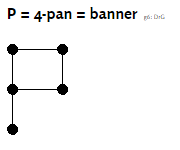
\includegraphics[scale=1]{figures/banner.png} 
		\caption[Đồ thị Banner]{Đồ thị Banner}
		\label{fig:banner}
	\end{figure}
\end{itemize}

Đồ thị $G'=(V',E')$ được gọi là đồ thị con \index{đồ thị con} của đồ thị $G=(V,E)$ nếu $V' \subseteq V$ và $E' \subseteq E$.

Ta gọi đồ thị $H$ là đồ thị con \textbf{cảm sinh} \index{cảm sinh} của đồ thị $G$ hay đồ thị $G$ cảm sinh $H$ nếu ta có thể thu được đồ thị $H$ bằng cách xóa đi một số đỉnh trong đồ thị $G$ (có thể không xóa đi đỉnh nào) cùng với những cạnh kề với các đỉnh đó.

Một đồ thị con của $G$ cảm sinh bởi một tập đỉnh $U \subset V(G)$ là đồ thị thu được bằng việc xóa đi tất cả các đỉnh của tập đỉnh $V(G) \setminus U$ trong đồ thị $G$, được kí hiệu là $G[U]$.

Cho một tập đỉnh $W \subset V(G)$, ta cũng nói rằng $W$ cảm sinh đồ thị $H$ nếu $G[W]$ cảm sinh $H$.

Ta kí hiệu $G - U := G[V(G) \setminus U]$ với $U \subseteq V(G)$.
Ta cũng kí hiệu $G - u := G - \{u\}$ với $u \in V(G)$.

\subsection{Alpha-dư thừa}
%Một đỉnh của đồ thị $G$ được gọi là $\alpha$-dư thừa nếu việc xóa đỉnh đó khỏi đồ thi $G$ không làm thay đổi số độc lập \index{số độc lập} của đồ thị $G$.
\begin{definition}
	\cite{alpharedundan} Cho đồ thị $G = (V,E)$, một đỉnh $v \in V(G)$ được gọi là $\alpha$-dư thừa ($\alpha$-redundant) \index{alpha-dư thừa} nếu $\alpha(G-v) = \alpha(G)$.
\end{definition}

Bài toán kiểm tra một đỉnh có phải là $\alpha$-dư thừa rõ ràng là tương đương với bài toán tìm tập độc lập cực đại, và do đó thuộc lớp bài toán NP-complete. Tuy nhiên trong một số trường hợp, những đỉnh $\alpha$-dư thừa có thể được nhận ra một cách hiệu quả.

\begin{lemma}
	\cite{alpharedudant2} Cho một đồ thị $G$ cảm sinh $K_{1,m}, \{u,v_1,v_2,...,v_m\}$, trong đó $u$ là đỉnh trung tâm (đỉnh có bậc $m$), sẽ tồn tại một số đỉnh $u_1,u_2,...,u_m$ sao cho $\{u,u_1,u_2,...,u_m\}$ là một tập độc lập và tồn tại một cặp ghép hoàn hảo giữa $\{u_i\}$ và $\{v_i\}$ hoặc $u$ là một đỉnh $\alpha$-dư thừa.
\end{lemma}

\subsection{Các thuật toán heuristic tham lam giải bài toán tìm tập độc lập cực đại}
Phương pháp heuristic có thể được sử dụng để tìm tập độc lập cực đại trong thời gian đa thức. Tôi sẽ tập trung vào những thuật toán heuristic tham lam để giải bài toán tìm tập độc lập cực đại.
%Tôi cũng sẽ đánh giá một số tính chất của những thuật toán này.

\subsubsection{Các phương pháp cổ điển}
Ta xem xét 3 thuật toán heuristic phổ biến cho bài toán tìm tập độc lập cực đại: MIN, MAX và VO (Vertex Ordering).

\paragraph{Thuật toán MIN}
\cite{MINAlgorithm} Thuật toán MIN \index{MIN} được mô tả như sau: bắt đầu với một tập độc lập rỗng $I$, thuật toán liên tiếp chọn những đỉnh có bậc nhỏ nhất trong $G$, thêm đỉnh này vào tập $I$ và xóa đỉnh đó đi khỏi đồ thị $G$. Thuật toán dừng khi đồ thị $G$ không còn có đỉnh nào.

%%%%%%%%%%%%%%%
\begin{algorithm}
	\caption{MIN($G$)}\label{MIN}
	\begin{algorithmic}[1]
		\INPUT Đồ thị $G$
		\OUTPUT Một tập độc lập cực đại của G.
		\State $I:= \emptyset$; $i:=1$; $H_i := G$;
		\While{$V(H_i) \neq \emptyset$}
			\State Chọn $u \in V(H_i)$ sao cho $\textrm{deg}_{H_i}(u) = \delta(H_i)$;
			\State $I := I \cup \{u\}$; $i:=i+1$; $H_i := H_{i-1} - N_{H_{i-1}}[u]$;
		\EndWhile
		\State \textbf{end while}
		\State \textbf{return} $I$
	\end{algorithmic}
\end{algorithm}
%%%%%%%%%%%%%%%
\paragraph{Thuật toán MAX}
Trong thuật toán MAX \index{MAX} \cite{MAXAlgorithm}, ta liên tiếp lựa chọn một đỉnh có bậc lớn nhất trong đồ thị $G$, xóa đỉnh đó khỏi $G$ cho đến khi $G$ không còn có cạnh nào nữa. Những đỉnh còn lại trên đồ thị hình thành một tập độc lập cực đại.

%%%%%%%%%%%%%%%
\begin{algorithm}
	\caption{MAX($G$)}\label{MAX}
	\begin{algorithmic}[1]
		\INPUT Đồ thị $G$
		\OUTPUT Một tập độc lập cực đại của G.
		\State $i:=n$; $H_i := G$;
		\While{$E(H_i) \neq \emptyset$}
			\State Chọn $u \in V(H_i)$ sao cho $\textrm{deg}_{H_i}(u) = \Delta(H_i)$;
			\State $i:=i - 1$; $H_i := H_{i+1} - u$;
		\EndWhile
		\State \textbf{end while}
		\State \textbf{return} $V(H_i)$
	\end{algorithmic}
\end{algorithm}
%%%%%%%%%%%%%%%
\paragraph{Thuật toán VO (Vertex Order)}
Trong thuật toán VO \index{VO} \cite{VOAlgorithm}, đầu tiên ta xắp xếp các đỉnh của đồ thị $G$ theo thứ tự tăng về bậc của đỉnh. Sau đó lần lượt xử lý các đỉnh trong danh sách đã được xắp xếp và thêm đỉnh vào tập độc lập nếu nó không kề với bất cứ đỉnh nào trong tập độc lập hiện tại.

%%%%%%%%%%%%%%%
\begin{algorithm}
	\caption{VO($G$)}\label{VO}
	\begin{algorithmic}[1]
		\INPUT Đồ thị $G$
		\OUTPUT Một tập độc lập cực đại của G.
		\State $I := \emptyset$;
		\State Sắp xếp tập đỉnh V(G) thành một danh sách tăng dần về bậc của đỉnh ($u_i$);
		\For {i:=1 \textbf{to} $n(G)$}
			\If {$N_I(u_i) = \emptyset$}
				\State $I:= I \cup \{u_i\}$;
			\EndIf
			\State \textbf{end if}					
		\EndFor
		\State \textbf{end for}
		\State \textbf{return} $I$
	\end{algorithmic}
\end{algorithm}
%%%%%%%%%%%%%%%

%\subsubsection{Cận Caro-Wei}
%Cho đồ thị $G$, ta kí hiệu $k_{MIN}(G)$, $k_{MAX}(G)$, và $k_{VO}(G)$ là lực lượng nhỏ nhất của tập độc lập cực đại đại được bằng thuật toán MIN, MAX, và VO. Wei[5] đã sử dụng thuật toán MIN để tìm ra cận dưới của $\alpha(G)$:
%$$
%\alpha(G) \geq k_{MIN}(G) \geq \sum_{v \in V(G)} \frac{1}{\textrm{deg}(v)+1}
%$$
%Caro[6] cũng độc lập chứng minh kết quả này. Griggs[3] cũng chỉ ra rằng thuật toán MAX có thể được sử dụng để chứng minh cận Caro-Wei.
%Ngoc C. Le et al.[2] đã chứng minh được một kết quả cho thuật toán VO:
%$$
%k_{VO}(G) \geq \sum_{v \in V(G)} \frac{1}{deg(v)+1}
%$$

\subsubsection{Phương pháp kết hợp}
Trong phần này, tôi sẽ mô tả một phiên bản được chỉnh sửa của thuật toán heuristic tham lam cổ điển. Thuật toán là sự kết hợp của thuật toán MIN và 
$\alpha$-dư thừa, được đề xuất bởi Ngoc C. Le et al. \cite{MIS}.

Ta có hệ quả sau rút ra từ bổ đề 4.1 trong trường hợp $m=2$.
\begin{corollary}
	Cho đồ thị $G = (V,E)$, một đỉnh $u \in V(G)$ là $\alpha$-dư thừa nếu tồn tại hai đỉnh $v_1, v_2 \in N(u)$ sao cho $v_1 \nsim v_2$ và không tồn tại hai đỉnh $u_1, u_2$ sao cho $\{u,u_1,u_2\}$ là độc lập và $\{u,u_1,u_2,v_1,v_2\}$ cảm sinh $K_{2,3}$ hoặc banner hoặc $P_5$.
\end{corollary}
%
\begin{figure}[!h]
	\centering
	\begin{subfigure}{.3\textwidth}
		\centering
		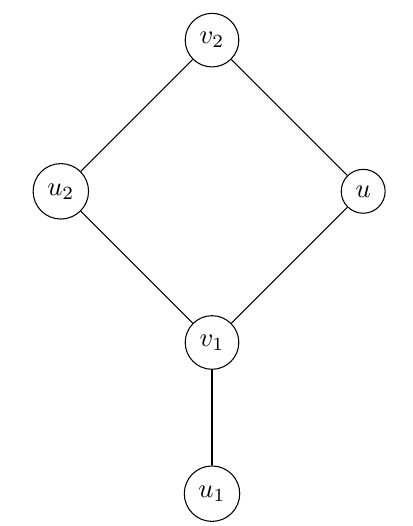
\includegraphics[scale=0.35]{figures/banner2.png}
		\caption{Banner}
		\label{fig:sub1}
	\end{subfigure}%
	\begin{subfigure}{.3\textwidth}
		\centering
		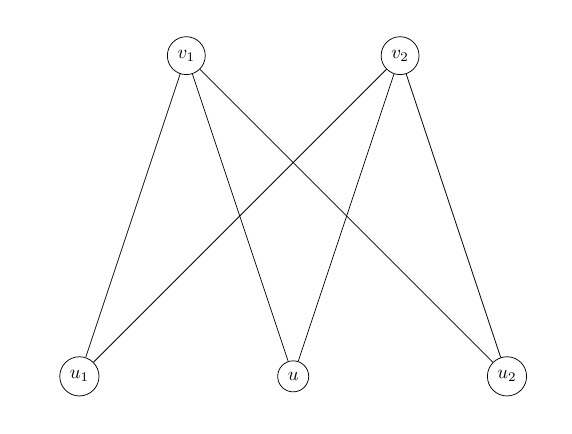
\includegraphics[scale=0.35]{figures/k23.png}
		\caption{$K_{2,3}$}
		\label{fig:sub2}
	\end{subfigure}
	\begin{subfigure}{.3\textwidth}
		\centering
		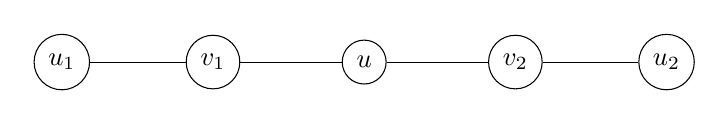
\includegraphics[scale=0.35]{figures/p5.png}
		\caption{$P_5$}
		\label{fig:sub2}
	\end{subfigure}
	\caption{Một số ví dụ minh họa trong đó  $v_1 \nsim v_2$, $\{u,u_1,u_2\}$ là độc lập và  $\{u,u_1,u_2,v_1,v_2\}$ cảm sinh đồ thị $ banner$, $K_{2,3}$ hoặc  $P_5$.}
	\label{fig:redundan}
\end{figure}
%
\paragraph{Thuật toán MMIN (Modified MIN)}
Thuật toán MMIN \index{MMIN} là sự kết hợp của kĩ thuật $\alpha$-dư thừa và thuật toán MIN.
Cho $G$ là một đồ thị đơn,vô hướng bất kỳ, gọi $n = |V(G)|$. Thuật toán liên tiếp lựa chọn một đỉnh có bậc nhỏ nhất là $u$, sau đó kiểm tra và xóa đỉnh $u$ nếu $u$ là $\alpha$-dư thừa bằng cách áp dụng hệ quả 4.0.1. 
Thuật toán MMIN trả về một tập độc lập cực đại.


%%%%%%%%%%%%%%%
\begin{algorithm}
	%\algsetup{linenosize=\Large}
	\caption{MMIN($G$)}\label{MMIN}
	\begin{algorithmic}[1]
		\INPUT Đồ thị $G$
		\OUTPUT Một tập độc lập cực đại của G.
		\State $I := \emptyset$; $i:=1$; $H_i=G$;
		\While {$V(H_i) \neq \emptyset$}
		\State Chọn $u \in V(H_i)$  sao cho $deg_{H_i}(u) = \delta(H_i)$;
		\ForAll {$v_1,v_2 \in N_{H_i}(u)$ sao cho $v_1 \nsim v_2$}
			\If {Không tồn tại $u_1,u_2 \in V(H_i)$ sao cho $\{u,u_1,u_2\}$ là độc lập và $\{u,u_1,u_2,v_1,v_2\}$ cảm sinh $P_5$ hoặc banner hoặc $K_{2,3}$}
				\State $H_{i+1} := H_i - u$; $i := i+1$;  \Comment{loại bỏ $u$ vì $u$ là $\alpha$-dư thừa}
				\State \textbf{Break};
			\EndIf
			\State \textbf{end if}
		\EndFor
		\State \textbf{end for}				
		\State $I := I \cup {u}$; $i := i+1$; $H_i := H_{i-1} - N_{i-1}[u]$;
		\EndWhile
	\State \textbf{end while}
	\State \textbf{return} $I$
	\end{algorithmic}
\end{algorithm}
%%%%%%%%%%%%%%%
%Cho một đồ thị đơn vô hướng bất kì $G$, gọi $n = |V(G)|$ thì thuật toán MMIN cho ra một tập độc lập cực đại. Ta có thể tìm ra đỉnh có bậc nhỏ nhất trong $G$ trong thời gian $O(n^2)$. Cho $(v_1,u,v_2)$ cảm sinh $P_3$, ta có thể kiểm tra liệu có tồn tại hai đỉnh $u_1, u_2$ sao cho $(u, u_1,u_2)$ là độc lập và $\{u,u_1,u_2,v_1,v_2\}$ cảm sinh $K_{2,3}$, banner, hoặc $P_5$ trong thời gian $O(n^2)$.

%Bài toán tìm tập độc lập có lực lượng hớn nhất và tính toán số độc lập của đồ thị có những ý nghĩa quan trọng trong nhiều lĩnh vực của đới sống, như lý thyết thông tin, sinh học, quản lý giao thông, viễn thông, v.v.\\
%Đầu tiên ta sẽ nhắc lại một số khái niệm cơ bản về lý thuyết đồ thị và tập độc lập, những định lý liên quan đến tập độc lập cực đại, và một số ứng dụng của bài toán tìm tập độc lập cực đại. 


\newpage
\fancyhead[R]{Ứng dụng bài toán tập độc lập cực đại trong dịch tễ học}
\section{Ứng dụng bài toán tập độc lập cực đại trong dịch tễ học}
\subsection{Giới thiệu về dịch tễ học}
Theo Bonita R, Beaglehole R, Kjellstrom K.\cite{BasicEpid}, \textbf{dịch tễ học}  \index{dịch tễ học} là khoa học nền tảng của y tế công cộng, được định nghĩa là "việc nghiên cứu sự phân bố của các yếu tố quyết định của các tình trạng hay sự kiện liên quan đến sức khỏe trong các quần thể xác định và việc ứng dụng những nghiên cứu này vào phòng ngừa và kiểm soát các vấn đề sức khỏe". 
Các nhà dịch tễ học không chỉ quan tâm đến tử vong, bệnh tật mà còn quan tâm tới cả trình trạng sức khỏe và quan trọng nhất là giải pháp tăng cường sức khỏe cho cộng đồng.

Trọng tâm của các nghiên cứu dịch tễ học là các quần thể xác định về địa lý hoặc các khía cạnh khác. Một quần thể dược đề cập trong dịch tễ học thường là quần thể được chọn từ một khu vực đặc thù vào một thời điểm cụ thể. Cấu trúc của các quần thể khác nhau ở các vùng địa lý khác nhau ở các thời điểm khác nhau có thể rất khác nhau. Nghiên cứu dịch tễ học rất quan tâm đến sự giao động này.

Dịch tễ học cùng với y học đã đạt được nhiều thành tựu không chỉ trong nghiên cứu mà còn trong thực tế, với những đóng góp lớn trong thanh toán các bệnh dịch lớn cũng như phát hiện nguyên nhân của nhiều căn bệnh trong xã hội. 
Một trong những thành tựu có thể kể đến là việc phát hiện ra rằng nhiễm khuẩn đậu bò sẽ góp phần bảo vệ chống virut đậu mùa, từ đó tìm ra cách giải quyết đại dịch trên toàn thế giới, hay tìm ra nguyên nhân gây ra bệnh Minamata tại Nhật Bản là do ô nhiễm môi trường gây nhiễm độc Methyl thủy ngân chứ không phải là một căn bệnh do nhiêm khuẩn.

\subsection{Dịch tễ học và lý thuyết đồ thị}
Lý thuyết đồ thị và dịch tễ học về các bệnh truyền nhiễm có mối liên kết chặt chẽ với nhau. Nền tảng của dịch tễ học và những mô hình dịch tễ dựa trên sự phân bố ngẫu nhiên của quần thể, nhưng trong thực tế, mỗi cá thể trong quần thể có quan hệ với một tập những cá thể khác, mà cá thể này có thể lây nhiễm hoặc bị lây nhiễm bệnh. Kết hợp các các mối quan hệ này lại, coi mỗi cá thể là một đỉnh của đồ thị và các quan hệ lây nhiễm là các cạnh giữa các đỉnh cho ta một mạng truyền nhiễm của quần thể.

Những kiến thức về cấu trúc của mạng truyền nhiễm cho phép tính toán những chỉ số trong mô hình dịch tễ học từ hành vi lây nhiễm của những cá thể. Những chỉ số về đồ thị của mạng truyền nhiễm trở nên quan trọng trong củng cố những hiểu biết và dự đoán về các mô thức truyền nghiễm và đo lường tác động của những can thiệp vào quần thể.

\subsection{Bài toán tìm tập độc lập cực đại và ứng dụng trong dịch tễ học}

Một trong những quan tâm của dịch tễ học là làm sao tiêm phòng cho một nhóm cá thể với số lượng ít nhất có thể, nhằm ngăn chặn sự lan rộng của bệnh truyền nhiễm, như ta có thể tham khảo trong hình \ref{fig:epidemiology}.

\begin{figure}[!h]
	\centering
	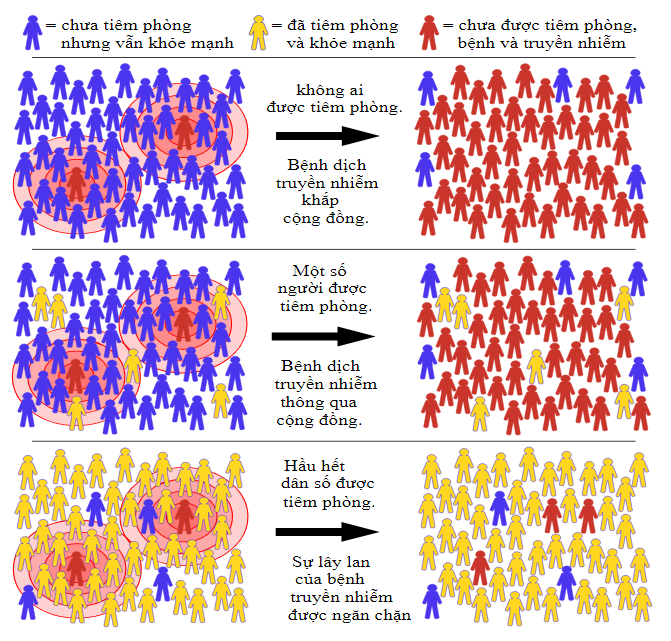
\includegraphics[scale=0.8]{figures/Herd_immunity_vn_2.png} 
	\caption[Mô tả tác động của việc tiêm phòng đến sự truyền nhiễm của bệnh dịch]{Mô tả tác động của việc tiêm phòng đến sự truyền nhiễm của bệnh dịch. Ta nhận thấy khi trong cộng đồng không có người được tiêm phòng (miễn nhiềm với bệnh dịch) thì bệnh dịch sẽ lan ra tự do. Khi chỉ có một số lượng nhỏ người được tiêm phòng cũng không ngăn được sự lan ra của bệnh dịch. Chỉ khi phần lớn cộng đồng được tiêm phòng, thì sự lan truyền của bệnh dịch mới được ngăn chặn (Nguồn: \href{https://en.wikipedia.org/wiki/Herd\_immunity}{Wikipedia}, đã được tôi dịch sang tiếng việt).}
	\label{fig:epidemiology}
\end{figure}

Dưới góc độ dịch tễ học, một cá thể đã tiêm phòng (miễn nhiễm với bệnh dịch) sẽ khó có thể bị mắc lại và cũng không thể trở thành cá thể trung gian lan truyền bệnh cho những cá thể khác được. 

Còn dưới góc độ của lý thuyết đồ thị, như đã đề cập trong phần 4.1, một tập đỉnh của đồ thị không có hai đỉnh nào kề nhau thì tập đỉnh này được gọi là tập độc lập. 

Vì vậy, nếu tìm được một tập những cá thể không có liên hệ trực tiếp với nhau trong mạng truyền nhiễm của quần thể (tập độc lập), ta chỉ cần tiêm phòng cho những cá thể còn lại của quần thể, thì kết quả là ta cô lập được những cá thể của tập cá thể độc lập (không có liên hệ trực tiếp), để họ không thể truyền nhiễm lẫn nhau được nữa và bệnh dịch được giải quyết.

Để giảm thiểu số cá thể phải tiêm phòng nhằm giảm chi phí cho xử lý bệnh dịch, ta cần cực đại hóa tập cá thẻ không có quan hệ trực tiếp trên, tức là quay trở về bài toán tìm tập độc lập cực đại trong đồ thị.
Đây chính là một ứng dụng đơn giản của lý thuyết đồ thị trong dịch tễ học.

Sau đây tôi sẽ trình bày kết quả thực hiện các thuật toán tìm tập độc lập đã đề cập trong phần 3, trên các bộ dữ liệu mạng cỡ lớn, là dữ liệu mạng giao thông của các thành phố trên thế giới, và đánh giá kết quả của các thuật toán.

\subsection{Nhận xét kết quả các thuật toán tìm tập độc lập cực đại trên các đồ thị cỡ lớn}

Từ kết quả chạy thuật toán trong bảng \ref{table:MIS}, ta có thể thấy kích thước của tập độc lập thu được là khá lớn so với kích thước của đồ thị, suy ra tập đỉnh còn lại cần phải "tiêm phòng" không quá lớn để đạt được hiệu quả ngăn chặn bệnh dịch lây lan ra cộng đồng.

Trong thực tế, mạng truyền nhiễm trong dịch tễ học có cấu trúc và nhiều tính chất khác với mạng giao thông, khi cấu trúc mạng giao thông thường phân tán, bán kính của đồ thị thường lớn, còn mạng truyền nhiễm lại phần nào giống với mạng xã hội, khi cả hai đều là tương tác giữa con người với con người. Nhưng vì thời gian có hạn, cũng như các dữ liệu mạng xã hội thường có kích thước rất lớn (từ vài triệu cho đến vài chục triệu đỉnh, hàng trăm triệu cạnh), các thuật toán được giới thiệu trong báo cáo này tuy là heuristic nhưng thời gian chạy vẫn chưa đủ nhanh. Nên trong báo cáo này, tôi chưa thể trình bày kết quả áp dụng các thuật toán tìm tập độc lập cực đại trên mạng xã hội được.
\newpage
\begin{table}[!h]
	\caption[Kết quả chạy các thuật toán tìm tập độc lập cực đại với các dữ liệu đường bộ]{Kết quả chạy các thuật toán tìm tập độc lập cực đại với các dữ liệu đường bộ của các thành phố trên thế giới. Cột thứ nhất là tên bộ dữ liệu, cụ thể ở đây là tên thành phố ứng với dữ liệu mạng giao thông của thành phố đó, cột thứ hai và thứ ba lần lượt là số đỉnh và số cạnh của đồ thị. Các cột còn lại là kích thước của tập độc lập tìm được ứng với mỗi thuật toán.}
	\centering
	\csvautotabular{MIS.csv}
	\label{table:MIS}
\end{table}

%%%%%%%%%%%%%%%%%%%%%%%%%%%%%%%%%%%%%%%%%%%%%%%%%%%%%%%%%%%%%%%%%%%%%%%%%%%%%%%%
\newpage
\fancyhead[R]{Lý thuyết đồ thị trong phân tích mạng giao thông vận tải}
\section{Lý thuyết đồ thị trong phân tích mạng giao thông vận tải}
Trong phần này của báo cáo, tôi sẽ trình bày một mô hình mạng giao thông vận tải đơn giản và giới thiệu các chỉ số thường được sử dụng trong phân tích mạng giao thông. 

\subsection{Các khái niệm trong giao thông vận tải}
Theo Wikipedia, \textbf{giao thông vận tải} \index{giao thông vận tải} là quá trình dịch chuyển của con người, và hàng hóa từ nơi này đến nơi khác, sử dụng những loại phương tiện vận tải và di chuyển trên hệ thống cơ sở hạ tầng giao thông. 

Giao thông vận tải đóng vai trò rất quan trọng trong xã hội hiện đại, vì nó cho phép sự trao đổi con người và hàng qua lại giữa khu vực, vốn là nguồn gốc sự phát triển của nền văn minh.

Những loại hình giao thông vận tải cơ bản gồm có: đường không, đường sắt, đường bộ, đường thủy, đường ống, dây cáp và đường hàng không vũ trụ. 

Những yếu tố cơ bản trong một hệ thống giao thông vận tải bao gồm: \textbf{cơ sở hạ tầng}, \textbf{phương tiện} và \textbf{vận hành}.
\begin{itemize}
	\item Cơ sở hạ tầng giao thông vận tải bao gồm sự xây dựng cố định của các loại đường đi như đường bộ, đường sắt, đường thủy, đường ống và các địa điểm đầu cuối như sân bay, nhà ga, kho hàng, cảng biển. Những địa điểm đầu cuối (terminal) có thể được sử dụng như nơi trung gian vận chuyển con người và hàng hóa hoặc là nơi lưu trữ.
	\item Phương tiện di chuyển ở trong giao thông vận tải rất đa dạng, từ đơn giản như đi bộ, phổ biến như xe ôtô, cho đến hiện đại như máy bay hay tàu vũ trụ.
	\item Vận hành hệ thống giao thông vận tải liên quan đến cách các phương tiện tham gia giao thông được điều khiển, liên quan đến những vấn đề khác như luật pháp, tài chính và các quy định. Trong ngành công nghiệp giao thông vận tải, cơ sở hạ tầng giao thông có thể được xây dựng để phục vụ mục đích công cộng hoặc do một tổ chức tư nhân đứng ra xây dựng và vận hành.
\end{itemize}

Hai chức năng chính của một hệ thống giao thông vận tải:
\begin{itemize}
	\item Vận tải hành khách, được chia ra hai loại là vận tải hành khách công cộng và vận tải hành khách tư nhân. Vận tải hành khách công cộng được lên kế hoạch trước về tuyến đường đi và thời gian, trong khi vận tải hàng khách tư nhân lại cung cấp dịch vụ vận chuyển linh động theo yêu cầu của khách hàng. Vận tải hành khách tư nhân cung cấp tính linh hoạt cao hơn, nhưng khả năng phục vụ thường thấp hơn, còn vận tải hành khách công cộng lại có khả năng phục vụ cao hơn và tác động xấu lên môi trường ít hơn.
	\item Vận tải hàng hóa, được coi là yếu tố then chốt trong chuỗi giá trị của sản xuất. Với sự phát triển của toàn cầu hóa, chuyên biệt hóa, nhu cầu vận chuyển hàng hóa đang càng ngày càng tăng cao. Khái niệm logistic ra đời để mô tả toàn bộ quá trình vận chuyển sản phẩm từ nhà sản xuất cho đến tận tay khách hàng.
\end{itemize}

Giao thông vận tải chính là chìa khóa của chuyên biệt hóa  (specialization) trong nền kinh tế, khi những khu vực kinh tế hay địa lý khác nhau, sản xuất những sản phẩm chuyên biệt của khu vực đó, lên một mức chuyên nghiệp và quy mô lớn, sau đó hàng hóa được vận chuyển và tiêu thụ ở khắp những khu vực khác trong nền kinh tế.

Ngoài những ảnh hưởng to lớn mà giao thông vận tải mang lại cho con người, cũng cần nhắc đến những tác động tiêu cực của nó lên môi trường. Trong thời đại công nghiệp hóa, giao thông vận tải sử dụng rất nhiều năng lượng, mà phần lớn là bắt nguồn từ năng lượng hóa thạch, vốn có tác động rất xấu đến môi trường, góp phần gây ra hiện tượng nóng lên toàn cầu.
Bằng những giải pháp mới trong công nghệ và điều hành hệ thống giao thông, chúng ta mong muốn có thể giảm thiểu được tác động của giao thông vận tải lên môi trường.


%Trong phần này của báo cáo, tôi sẽ trình bày quá trình xây dựng mô hình đồ thị cho mạng giao thông quốc lộ của Việt Nam, với nguồn là dữ liệu GIS về các đường quốc lộ. Từ mô hình đồ thị, tôi đo lường một số chỉ số về độ phân cụm của mạng, độ trung tâm của những nút trong mạng, tính hiệu quả của mạng, từ đó đưa ra phân tích về tình trạng giao thông tại Việt Nam.

\subsection{Mô hình mạng giao thông vận tải bằng đồ thị}

Bản chất của hệ thống giao thông vận tải đã cho thấy sự phù hợp khi mô hình bằng đồ thị. Trong bất cứ hệ thống giao thông vận tải nào cũng đều có các địa điểm đầu cuối (terminal), nơi bắt nguồn, trung gian và kết thúc của luồng phương tiện di chuyển, ví dụ như các sân bay trong vận chuyển hàng không, các ga trong vận tải đường sắt, các kho hàng trong giao thông đường bộ, các cảng biển trong giao thông đường thủy, đều là các địa điểm đầu cuối. Một cách đơn giản, ta có thể coi các địa điểm đầu cuối của hệ thống giao thông vận tải là các đỉnh của đồ thị, và các đường đi trong cơ sở hạ tầng chính là cạnh nối các đỉnh này lại với nhau.

Trong thực tế, có rất nhiều cách khác nhau để mô hình một mạng giao thông vận tải, và mô hình được lựa chọn phụ thuộc vào bài toán đặt ra. 
Đối với bài toán tìm đường đi ngắn nhất hay định tuyến trên mạng giao thông đường bộ, thì coi mỗi nút giao thông là một đỉnh, mỗi đoạn đường là một cạnh của đồ thị là một cách mô hình hợp lý. 
Nhưng đối với bài toán tìm những tuyến đường có mật độ giao thông cao, hay xảy ra ùn tắc thì ta có thể coi mỗi một đoạn đường là một đỉnh của đồ thị, và hai đỉnh có cạnh nối với nhau nếu chúng giao nhau tại một nút giao thông nào đó.

Trong báo cáo này, tôi sẽ sử dụng mô hình mạng giao thông phổ biến nhất, coi mỗi nút giao thông là một đỉnh và mỗi đoạn đường là một cạnh nối hai nút giao thông với nhau.
\subsection{Các chỉ số trong phân tích đồ thị}
%%%%

\subsubsection{Khoảng cách, tâm sai, bán kính, đường kính và mật độ của đồ thị}

Một trong những bài toán của phân tích đồ thị là quyết định độ quan trọng của một đỉnh hay một cạnh. Chỉ số \textbf{tính trung tâm} \index{tính trung tâm} (centrality) của một đỉnh hoặc một cạnh trong đồ thị thường chỉ ra mức độ ảnh hưởng của một đỉnh đó đến toàn bộ đồ thị. Có rất nhiều loại chỉ số trung tâm khác nhau và mỗi chỉ số có cách tính cũng như ý nghĩa khác nhau trong đánh giá độ quan trọng của một đỉnh hay cạnh của đồ thị.

Trước khi đề cập đến các chỉ số trung tâm (centrality), ta sẽ nhắc lại một số khái niệm cơ bản về lý thuyết đồ thị được sử dụng trong phần này.

\cite{graphtextbook} Cho đồ thị $G=(V,E)$, \textbf{khoảng cách} \index{khoảng cách} giữa hai đỉnh $u$ và $v$ của đồ thị $G$ là độ dài của đường đi ngắn nhất giữa hai đỉnh. Khoảng cách này kí hiệu là $d(u,v)$.

\cite{graphtextbook} \textbf{Tâm sai} \index{Tâm sai} (eccentricity) của một đỉnh trong một đồ thị liên thông là khoảng cách lớn nhất từ một đỉnh đến các đỉnh khác của đồ thị:
\begin{equation}
\sigma(v) = \max_{u \in v} d(u,v)
\end{equation}

\cite{graphtextbook} Đường kính của đồ thị liên thông $G$, kí hiệu là $diam(G)$ là khoảng cách lớn nhất giữa hai đỉnh của đồ thị. Công thức tính đường kính của đồ thị:
\begin{equation}
diam(G) = \max_{v \in V} \sigma(v)
\end{equation}

\cite{graphtextbook} Bán kính của đồ thị liên thông $G$ là giá trị nhỏ nhất của tâm sai của một đỉnh trong các đỉnh của đồ thị:
\begin{equation}
rad(G) = \min_{v \in V} \sigma(v)
\end{equation}

\cite{graphtextbook} Mối quan hệ giữa bán kính và đường kính của đồ thị $G$:
\begin{equation}
rad(G) \leq diam(G) \leq 2 * rad(G)
\end{equation}

\cite{complexnetwork} Mật độ của đồ thị $G=(V,E)$, kí hiệu là $\rho(G)$, là tỉ lệ giữa số cạnh của đồ thị và số cạnh của một đồ thị đầy đủ có cùng số đỉnh:
\begin{equation}
\rho(G) = \frac{2m}{n(n-1)}
\end{equation}

Nếu mật độ của đồ thị không thay đổi nhiều khi $n \rightarrow \infty$ thì đồ thị được gọi là đồ thị dày (dense graph). Ngược lại, nếu $\rho \rightarrow 0$ khi $n \rightarrow \infty$ thì đồ thị được gọi là đồ thị thưa (sparse graph).

\subsubsection{Phân phối bậc}
Vẽ biểu đồ quan hệ giữa số bậc của đỉnh và số lượng đỉnh có bậc đó cho ta phân bố bậc của đồ thị. Phân phối bậc $P(k)$ của một đồ thị vô hướng $G$ là xác suất có một đỉnh nào đó của đồ thị có bậc là $k$.
\begin{definition}
	Phân phối bậc $P(k)$ của bậc $k$ trong đồ thị $G$ được tính bằng tỉ lệ giữa số đỉnh bậc $k$ trong $G$ trên tổng số đỉnh của đồ thị.
	\begin{equation}
	P(k) = \frac{n_k}{n}
	\end{equation}
\end{definition}
\subsubsection{Hệ số phân cụm}
\begin{definition}
	\cite{complexnetwork}Cho đồ thị $G = (V,E)$, hệ số phân cụm \index{hệ số phân cụm} của một đỉnh $v \in V(G)$ kí hiệu là $cc(v)$ được định nghĩa là tỉ lệ giữa số cạnh tồn tại giữa các lân cận của đỉnh $v$ và số cạnh tối đa có thể có giữa những lân cận. Ta có công thức:
	\begin{equation}
	cc(v) = \frac{2m_v}{n_v(n_v-1)}
	\end{equation}
	trong đó $n_v$ là số đỉnh lân cận của đỉnh $v$ và $m_v$ là số cạnh giữa các lân cận của đỉnh $v$.
\end{definition}

Hệ số phân cụm $cc(v)$ trên được gọi là hệ số phân cụm địa phương. Hệ số phân cụm trung bình $CC(G)$ của đồ thị $G$ là trung bình giá trị của hệ số phân cụm của tất cả các đỉnh trong đồ thị:
\begin{equation}
CC(G) = \frac{1}{n}\sum_{v \in V}cc(v)
\end{equation}
Một hệ số phân cụm trung bình thấp cho thấy tính liên kết kém giữa các cặp đỉnh của đồ thị. Nói cách khác, $CC(G)$ cho thấy độ dầy đặc của đồ thị.

Một phương pháp khác để tính hệ số phân cụm là sử dụng đồ thị tham giác và đồ thị bộ ba (triad). Đồ thị tam giác là đồ thị $K_3$, đồ thị bộ ba là đồ thị $P_3$. Ta có thể nhận thấy rằng số đồ thị tam giác mà một đỉnh kề với, chính là số cạnh giữa các đỉnh lân cận của đỉnh đó, số đồ thị bộ ba mà một đỉnh kề với, chính là số cạnh tối đa có thể có giữa các đỉnh lân cận của đỉnh đó.
Dựa trên điều này, ta có công thức khác tính hệ số phân cụm của một đỉnh:
\begin{equation}
cc(v) = \frac{n_t(v)}{n_x(v)}
\end{equation}
với $n_t(v)$ và $n_x(v)$ lần lượt là số đồ thị tam giác và số đồ thị bộ ba ứng với đỉnh $v$ của đồ thị.

\begin{definition}
	\cite{complexnetwork} Cho một đồ thị đơn liên thông $G = (V,E)$ và $n_t(G)$ là số đồ thị tam giác phân biệt trong $G$, $n_t(G)$ là số đồ thị bộ ba phân biệt trong $G$. Hệ số bắc cầu \index{Hệ số bắc cầu} (network transitivity) của đồ thị $G$, $\tau(G)$ là tỉ lệ giữa $n_t(G)$ và $n_x(G)$, có công thức.
	\begin{equation}
	\tau(G) = \frac{3n_t(G)}{n_x(G)} = \frac{\sum n_t(v)}{\sum n_x(v)}
	\end{equation}
	Sở dĩ có số 3 trong công thức vì mỗi đỉnh của đồ thị tam giác được tính một lần trong $n_x(G)$.
\end{definition}

\begin{figure}[!h]
	\centering
	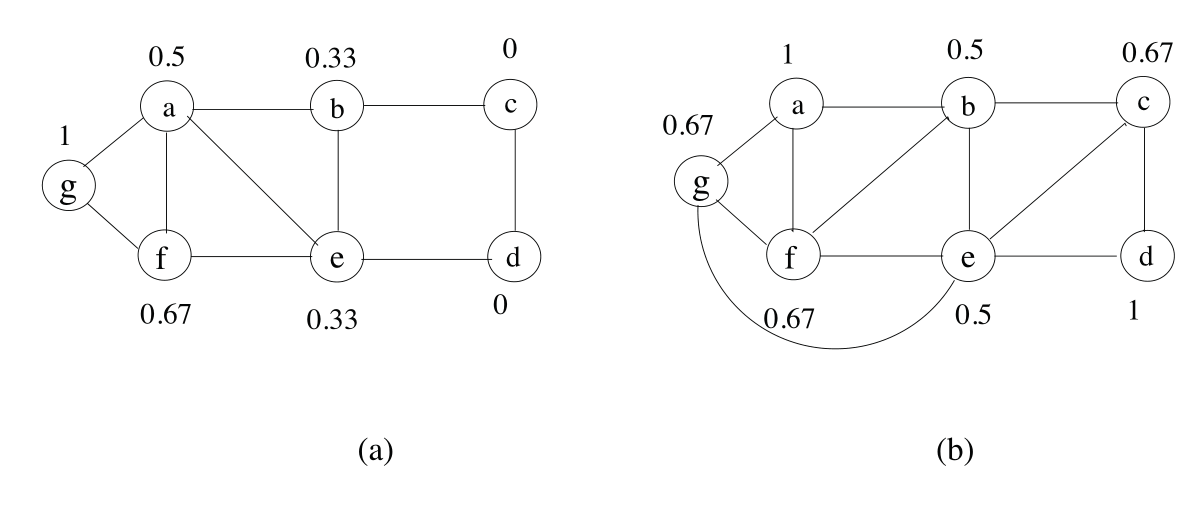
\includegraphics[scale=0.5]{figures/clustercoefficient.png} 
	\caption[Hệ số phân cụm]{Hệ số phân cụm của đồ thi (a) là 0.4 trong khi hệ số phân cụm của đồ thị (b) là 0.71, thể hiện rằng đồ thị (b) dày đặc hơn và có kết nối với nhau nhiều hơn.}
	\label{fig:clustercoeff}
\end{figure}

\subsubsection{Chỉ số trung tâm bậc và chỉ số trung tâm gần gũi}
Chỉ số trung tâm bậc (degree centrality) dựa trên ý tưởng rằng một đỉnh quan trọng thì có bậc hay số đỉnh kề với nó cao. Cho đồ thị $G=(V,E)$, $|V(G)| = N$, công thức chuẩn hóa của chỉ số trung tâm bậc của đỉnh $i$ trong đồ thị $G$, $C_D(i)$ được định nghĩa bởi Freeman \cite{centrali01},\cite{centrali02}:
\begin{equation}
C_D(i) = \frac{k_i}{N-1} = \frac{\sum_{j \in N}a_{ij}}{N-1}
\end{equation}
trong đó $k_i$ là số cạnh $(i,j)$ nối đỉnh $i$ với các đỉnh khác của đồ thị, $a_{ij}$ là giá trị của ô $(i,j)$ trong ma trận kề biểu diễn cho đồ thị $G$.

Đối với đồ thị mạng giao thông (không kể đến mạng giao thông hàng không) thì chỉ số trung tâm bậc bị giới hạn bởi không gian, khi coi các đỉnh là các điểm nút giao thông, bậc của các đỉnh trong đồ thị này thường thấp (số lượng ngã 5, ngã 6 thường rất ít trong mạng giao thông thực tế).

Chỉ số trung tâm gần gũi (closeness centrality measure) được đề xuất bởi Sabidussi \cite{centrali03} là nghịch đảo của khoảng cách trung bình từ đỉnh i đến mọi đỉnh khác trong đồ thị, có công thức chuẩn hóa:
\begin{equation}
C_C(i) = \frac{N-1}{\sum_{j \in V} d(i,j)}
\end{equation}
trong đó $d(i,j)$ là khoảng cách giữa hai đỉnh $i$ và $j$.

Vì trong đồ thị, chỉ số trung tâm gần gũi phụ thuộc rất nhiều vào vị trí của đỉnh, đo đó trong mạng giao thông, các đỉnh ở vị trí trung tâm địa lý chắc chắn sẽ có chỉ số trung tâm gần gũi cao.
\subsubsection{Chỉ số trung tâm trung gian}
Chỉ số \textbf{trung tâm trung gian} \index{trung tâm trung gian} (betweeness centrality) của một đỉnh là số đường đinh ngắn nhất giữa tất cả các đỉnh mà có đi qua đỉnh đó \cite{centrali02}. Công thức của chỉ số trung tâm trung gian được chuẩn hóa:
\begin{equation}
C_B(i) = \frac{1}{(N-1)(N-2)} \sum_{j,k \in V(G); j \neq k; k\neq i; j \neq i} \frac{n_{jk}(i)}{n_{jk}}
\end{equation}
trong đó $n_{jk}$ là tổng số đường đi ngắn nhất giữa hai đỉnh $j$ và $k$, $n_{jk}(i)$ là số đường đi ngắn nhất giữa hai đỉnh $j$ và $k$ mà có đi qua đỉnh i.

Công thức $C_B(i)$ trên đã được chuẩn hóa và đạt giá trị cao nhất là 1 khi mọi đường đi ngắn nhất trong đồ thị đều chứa đỉnh $i$. Một định nghĩa tương tự chỉ số trung tâm trung gian cho cạnh cũng có thể được định nghĩa.

\subsubsection{Chỉ số trung tâm hiệu quả và chỉ số trung tâm thẳng}
Bắt nguồn từ ý tưởng rằng hiệu quả của một mạng giao thông có thể được tính bằng việc so sánh độ dài của đường đi ngắn nhất giữa các đỉnh và khoảng cách chim bay (crowfly distance) giữa các đỉnh đó \cite{efficiency01}, chỉ số trung tâm hiệu quả (efficiency centrality) $C_E(i)$ và chỉ số trung tâm thẳng (straightness centrality) $C_S(i)$ được định nghĩa \cite{efficiency02}:
\begin{equation}
C_S(i) = \frac{1}{N-1} \mathlarger{\sum}_{j \in V(G); j \neq i} \frac{d^{\text{crowfly}}(i,j)}{d(i,j)}
\end{equation}
\begin{equation}
C_E(i) = \frac{\mathlarger{\sum}_{j \in V(G); j \neq i}\frac{1}{d(i,j)}}{\mathlarger{\sum}_{j \in V(G); j \neq i}\frac{1}{d^{\text{crowfly}}(i,j)}}
\end{equation}
trong đó $d^{\text{crowfly}}(i,j)$ là khoảng cách chim bay giữa hai đỉnh $i$,$j$ của mạng.

Ta có thể thấy rằng khi khoảng cách giữa một đỉnh và các đỉnh còn lại trong đồ thị càng lớn, thì chỉ số trung tâm hiệu quả và chỉ số trung tâm thẳng của đỉnh đó càng thấp.
%%%%
\newpage
\fancyhead[R]{Ứng dụng đồ thị vào phân tích mạng giao thông Việt Nam}
\section{Ứng dụng đồ thị vào phân tích mạng giao thông Việt Nam}
\subsection{Cơ bản về khoa học thông tin địa lý (GIS) và các mô hình dữ liệu địa lý}

Khái niệm GIS thường được hiểu là viết tắt của Geographical Information System, tức hệ thống thông tin địa lý, là một hệ thống máy tính, lưu trữ, xử lý và hiển thị dữ liệu địa lý.

GIS cũng có thể được hiểu là Geographical Information Sciences, tức khoa học về thông tin địa lý. Trong cáo cáo này, GIS được mặc định là viết tắt của khoa học thông tin địa lý.

\subsubsection{Các khái niệm cơ bản trong GIS}
\textbf{Hệ thống thông tin địa lý} \index{Hệ thống thông tin địa lý} là một tập hợp có tổ chức, bao gồm hệ thống phần cứng, phần mềm máy tính, dữ liệu địa lý và con người, được thiết kế nhằm mục đích nắm bắt, lưu trữ, cập nhật, điều khiển, phân tích, và hiển thị tất cả các dạng thông tin liên quan đến vị trí địa lý.

Các thành phần chính cấu thành nên một hệ thống thông tin địa lý:
\begin{itemize}
	\item Phần cứng hay chính là hệ thống máy tính có khẳ năng tính toán cũng như lưu trữ dữ liệu của hệ thống thông tin địa lý.
	\item Phần mềm, là các chương trình được viết ra để thực hiện các chức năng của một hệ thống thông tin địa lý.
	\item Dữ liệu của hệ thống thông tin địa lý gồm có dữ liệu không gian hay dữ liệu địa lý, mô tả các thuộc tính về không gian và địa lý của các đối tượng trên trái đất, dữ liệu phi thuộc tính hay dữ liệu phi không gian, cung cấp thêm các thông tin định tính và định lượng khác liên quan đến đối tượng.
	\item Phương pháp, là các mô hình của dữ liệu địa lý, cùng những kĩ thuật xử lý dữ liệu dựa trên mô hình này để thu được những tri thức mới.
	\item Con người đóng vai trò quan trọng trong tất cả các hoạt động của hệ thống thông tin địa lý.
\end{itemize}

Các chức năng chính của một hệ thống thông tin địa lý:
\begin{itemize}
	\item Thu thập dữ liệu, là công việc khó khăn trong quá trình xây dựng một hệ thống thông tin địa lý. Các dữ liệu thu thập từ được có thể từ nhiều nguồn khác nhau, từ dữ liệu địa lý đo đạc thực địa cho đến dữ liệu thống kê.
	\item Xử lý dữ liệu, cũng là bước khó khăn không kém, khi nguồn dữ liệu rất đa dạng, có rất nhiều vấn đề phải đối mặt để xử lý dữ liệu, thống nhất định dạng trước khi đưa vào hệ thống như: mất mát dữ liệu của một số đối tượng, dữ liệu có nhiễu và sai số, các nguồn dữ liệu không khớp nhau, v.v.
	\item Quản lý dữ liệu là chức năng cơ bản của hệ thống thông tin địa lý. Khi khối lượng dữ liệu trở nên lớn hay cực lớn, thì bài toán sắp xếp dữ liệu sao cho hợp lý, truy vấn và xử lý sao cho hiệu quả trở nên không đơn giản.
	\item Hiển thị dữ liệu, tức là cho phép hiển thị dữ liệu lên cho người dùng, dưới các dạng khác nhau như dữ liệu trên bản đồ hay các biểu đồ tổng hợp dữ liệu.
	\item Phân tích dữ liệu và trả lời các câu hỏi đặt ra về dữ liệu địa lý.
\end{itemize}

Cùng với sự ra đời của những hệ thống thông tin địa lý, ngành khoa học về thông tin  địa lý cũng ra đời, đóng góp những khái niệm và những tiêu chuẩn trong cách thức hoạt động của các hệ thống thông tin địa lý.

Sau đây là một số khái niệm cơ bản cần được đề cập đến trước khi nói về những loại dữ liệu GIS.
\begin{itemize}
	\item \textbf{Vị trí} (location) địa lý trong GIS thể hiện tọa độ của những điểm trên bề mặt của trái đất. Một cách thông thường trong đo lường vị trí trên trái đất là sử dụng hệ tọa độ kinh độ-vĩ độ.	
	\item \textbf{Khoảng cách} (distance) trong GIS có nhiều loại khác nhau, có khoảng cách góc, khoảng cách tuyến tính hay khoảng cách theo đường chim bay và khoảng cách đường đi. Mỗi một loại khoảng cách lại có đơn vị đo của chúng.
	\item \textbf{Phép chiếu} (projection) là một biến đổi toán học, giúp tạo ra bản đồ hai chiều của trái đất từ không gian ba chiều. Những phép chiếu nổi tiếng: phép chiếu Mercator, phép chiếu UTM.
	Có hàng trăm phép chiếu khác nhau được phát triển, và không có phép chiếu nào là hoàn hảo, luôn có sự sai lệch trong biểu diễn bản đồ. Một số bản đồ giúp bảo toàn diện tích nhưng lại làm biến dạng hình dạng của đối tượng địa lý, ngược lại có những bản đồ bảo toàn hình dạng của đối tượng địa lý nhưng lại sai về diện tích.
	\item \textbf{Hệ tọa độ địa lý} (coordinate system) cho phép biểu diễn vị trí của các điểm trên trái đất trong một hệ tọa độ, thường liên quan đến phép chiếu và các quy định về kích thước và hình dạng của trái đất. Ví dụ một hệ tọa độ địa lý thường sử dụng là UTM (Universal Transverse Mercator), chia thế giới thành 60 vùng khác nhau, mỗi vùng có một phép chiếu khác nhau để làm giảm sai lệch của phép chiếu trong tính toán.		
\end{itemize}
\subsubsection{Các loại dữ liệu cơ bản trong GIS}
%%%
Trong khoa học thông tin địa lý, để biểu diễn các đối tượng địa lý trong thực tế, người ta phải sử dụng các \textbf{mô hình dữ liệu} \index{mô hình dữ liệu},trong đó chỉ xem xét một khía cạnh nào đó của đối tượng.

Một số mô hình dữ liệu thông thường trong các hệ thống thông tin địa lý:
\begin{itemize}
	\item Mô hình dữ liệu vector, trong đó các đối tượng được biểu diễn như các \textbf{điểm} (point), \textbf{đường} (polyline) hay các \textbf{đa giác} (polygon). Ví dụ như một hồ nước có thể được mô hình dưới dạng một đa giác biểu diễn biên của nó, hay một cây có thể được biểu diễn như điểm, đường cao tốc có thể biểu diễn như đường (tức là một tập các điểm).
	\item Mô hình dữ liệu raster, là một ma trận các điểm ảnh lưu trữ những thông tin địa lý.
	\item Mô hình TIN (Triangulated Irregular Network) biểu diễn dữ liệu như một tập các tam giác kề nhau và không chồng lên nhau.
	\item Còn nhiều loại mô hình dữ liệu khác, nhưng hai loại mô hình dữ liệu vector và raster là được sử dụng nhiều nhất và cũng phổ biến nhất. Xem ví dụ về các mô hình dữ liệu của cùng một đối tượng vật lý, hình \ref{fig:rastervector}.
\end{itemize}

\begin{figure}[!h]
	\centering
	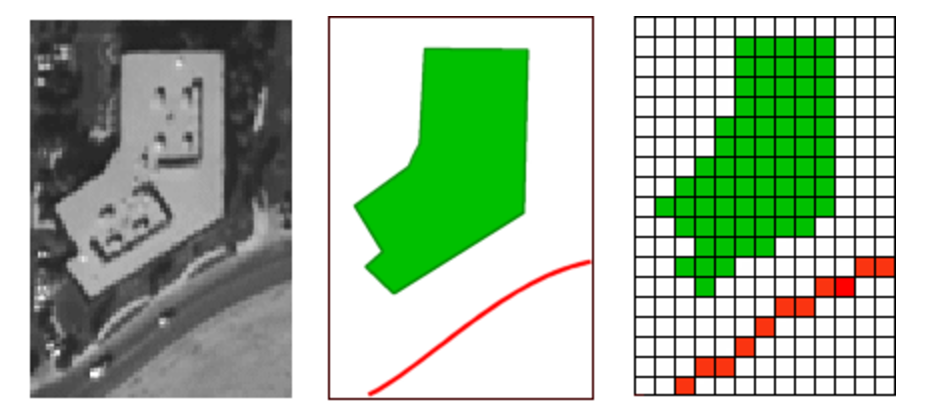
\includegraphics[scale=0.6]{figures/datamodelexample.png} 
	\caption[Mô hình dữ liệu vector và raster của đối tượng]{Mô hình dữ liệu vector và raster của đối tượng. Hình ở giữa là mô hình vector, trong đó ngôi nhà được coi là một đa giác, còn đường đi được coi là một đường. Hình ở bên phải là mô hình raster, trong đó tất cả đối tượng chỉ là tập hợp của các điểm ảnh (Nguồn: \href{http://www.geography.hunter.cuny.edu/~jochen/GTECH361/lectures/lecture05/concepts/03\%20-\%20Geographic\%20data\%20models_files/image003.gif}{geography.hunter.cuny.edu}).}
	\label{fig:rastervector}
\end{figure}
%%%

\subsubsection{Mô hình dữ liệu vector}
Mô hình dữ liệu vector bắt nguồn từ khái niệm đồ họa Vector trong đồ họa máy tính, khi các đối tượng được biểu diễn bằng danh sách các điểm, khi nối các điểm lại với nhau ta được hình dạng của đối tượng.

Ba loại hình học cơ bản được định nghĩa để biểu diễn đối tượng trong mô hình dữ liệu vector là: điểm, đường và đa giác.

Dữ liệu diểm thực chất là tọa độ của một điểm trên trái đất. Dữ liệu đường là một danh sách có thứ tự các dữ liệu điểm. Dữ liệu đa giác là dữ liệu đường trong đó điểm đầu và điểm cuối của danh sách trùng nhau.

Trong khoa học thông tin địa lý, một cấu trúc phân cấp được thiết kế để lưa trữ những dữ liệu dạng vector này, cấu trúc này được mô tả trong hình \ref{fig:vectordata}.

\begin{figure}[!h]
	\centering
	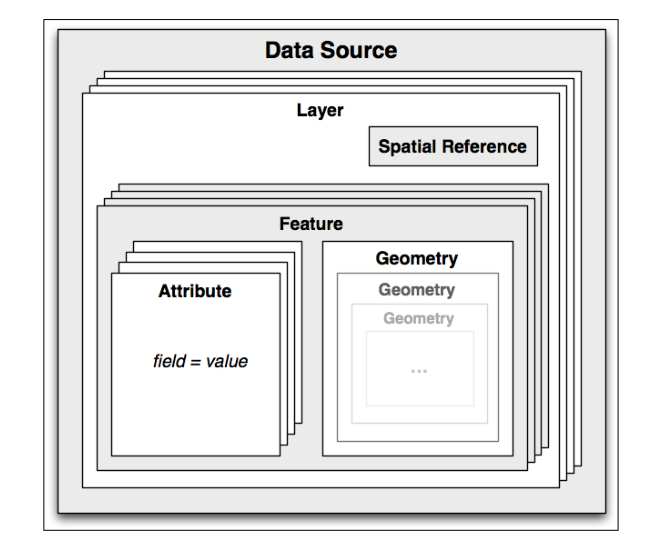
\includegraphics[scale=0.6]{figures/vectordataformat.png} 
	\caption[Cấu trúc lưu trữ dữ liệu dạng vetor.]{Cấu trúc lưu trữ dữ liệu dạng vector\cite{geospatialbook}.}
	\label{fig:vectordata}
\end{figure}

Trong cấu trúc lưu trữ dữ liệu vector này, lớp ngoài cùng là nguồn dữ liệu (data source), thường ứng với một tệp được lưu trữ.

Trong một nguồn dữ liệu có thể có một hay nhiều lớp dữ liệu (layer), mỗi lớp dữ liệu sẽ có một tham chiếu về hệ tọa độ không gian (spatial reference), định nghĩa hệ tọa độ không gian mà dữ liệu này sử dụng để mô tả đối tượng.

Mỗi một lớp lại bao gồm các đặc trưng (feature). Mỗi đặc trưng đại diện cho một đối tượng vật lý trong thực tế. Đối tượng này được biểu diễn thông qua một tập những đối tượng hình học (geometry). Đối tượng hình học này thuộc một trong 3 loại đối tượng: điểm, đường và đa giác.

Mỗi đặc trưng hay đối tượng sẽ đi liền với một tập dữ liệu phi không gian, biểu diễn dưới dạng các trường dữ liệu như trong bảng cơ sở dữ liệu.

Trong báo cáo này, dữ liệu đường bộ Việt Nam được sử dụng để xây dựng mạng đường bộ cũng là dữ liệu vector.

\subsubsection{Phần mềm QGIS}
\cite{qgis} QGIS hay QuantumGIS là phần mềm mã nguồn mở về hệ thống thông tin địa lý, là một công cụ hỗ trợ đắc lực những người làm về GIS, bằng hệ thống tính năng hoàn chỉnh cũng như khả năng mở rộng thông qua các tình cắm (plugin).
QGIS đem lại một môi trường làm việc với các hệ thống thông tin địa lý cho mọi đối tượng có nhu cầu sử dụng.

QGIS đem đến các tính năng nổi bật như:
\begin{itemize}
	\item hiển thị các loại dữ liệu liên quan đến hệ thống thông tin địa lý, hỗ trợ đọc và ghi nhiều chuẩn dữ liệu của các phần mềm GIS khác như ArcMap hay MapInfo. GGIS cũng cho phép tùy chỉnh cách hiển thị dữ liệu, cho phép hiển thị nhiều lớp dữ liệu chồng lên nhau trên cùng một bản đồ.
	\item Cho phép truy cập cơ sở dữ liệu của các hệ thống thông tin địa lý và hiển thị ra như những tệp dữ liệu thông thường.
	\item Kết hợp với các thư viện và công cụ xử lý dữ liệu mã nguồn mở khác, cung cấp rất nhiều thuật toán xử lý dữ liệu GIS.
	\item Công cụ chỉnh sửa và xây dựng bản đồ cho những nhà làm bản đồ.
\end{itemize}

Trong báo cáo này, một số hình ảnh về dữ liệu đường bộ Việt Nam được hiển thị bởi phần mềm QGIS.

\subsubsection{Phầm mềm Gephi}
\cite{gephi} Gephi là phần mềm mã nguồn mở giúp hiển thị trực quan, phân tích và khám phá trên dữ liệu đồ thị có kích thước rất lớn.
Những tính năng chính của Gephi:
\begin{itemize}
	\item Hiển thị đồ thị trực quan và có thể tương tác được.
	\item Sắp xếp cách hiển thị đồ thị (layout) với các thuật toán như Random Layout hay OpenOrd.
	\item Cung cấp các công cụ và thuật toán phân tích đồ thị, như PageRank, HITS,...
	\item Cung cấp công cụ thao tác trên các trường dữ liệu ứng đỉnh và các cạnh của đồ thị.
	\item Hỗ trợ đồ thị động thay đổi theo thời gian.
	\item Nhiều trình cắm hữu ích hỗ trợ.
	\item Khả năng tạo ra những kết quả biểu diễn đồ thị tùy chỉnh đẹp.
\end{itemize}
Tôi đã sử dụng Gephi để tính toán một số chỉ số trên đồ thị đường bộ Việt Nam, cũng như xuất những kết quả hiển thị đồ thị có tùy chỉnh với chất lượng tốt.

\subsubsection{Thư viện NetworkX}
\cite{neworkx} Thư viện NetworkX là thư viện mã nguồn mở, viết bằng ngôn ngữ lập trình Python cung cấp các hàm thao tác trên dữ liệu đồ thị, như tạo, chỉnh sửa, lưu và đặc biệt là có nhiều thuật toán về phân tích đồ thị, như sinh đồ thị ngẫu nhiên, phân cụm đồ thị, tính toán các thông số của đồ thị và còn nhiều tính năng khác nữa.

Cấu trúc dữ liệu đồ thị trong thư viện NetworkX cũng rất linh động, hỗ trợ nhiều kiểu đồ thị khác nhau. Vì được viết bằng ngôn ngữ lập trình Python nên thư viện NetworkX rất dễ dùng, đơn giản và lại có rất nhiều thuật toán tốt.

Thư viện NetworkX được tôi sử dụng đẻ tính toán phần lớn các kết quả cũng như lập trình các thuật toán trong báo cáo này.
\subsection{Xây dựng mạng giao thông đường bộ Việt Nam sử dụng dữ liệu GIS}
\subsubsection{Dữ liệu GIS về giao thông đường bộ Việt Nam}
Dữ liệu GIS đường bộ Việt Nam được sử dụng trong báo cáo này mô tả các trục đường quốc lộ trên toàn quốc, và là dữ liệu của năm 2008. (hình \ref{fig:vnhighway01} và \ref{fig:vnhighway02}).
\begin{figure}
	\centering
	\begin{minipage}{0.7\textwidth}
		\centering
		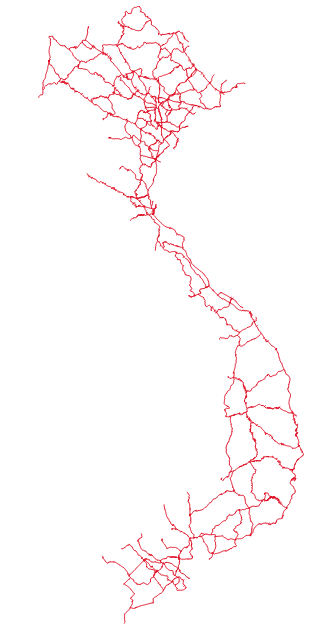
\includegraphics[width=0.5\textwidth]{figures/vietnamroad.png} % first figure itself
		\caption[Dữ liệu đường bộ Việt Nam]{dữ liệu đường bộ Việt Nam, hiển thị bằng phần mềm QGIS.}
		\label{fig:vnhighway01}
	\end{minipage}\hfill
	\begin{minipage}{0.7\textwidth}
		\centering
		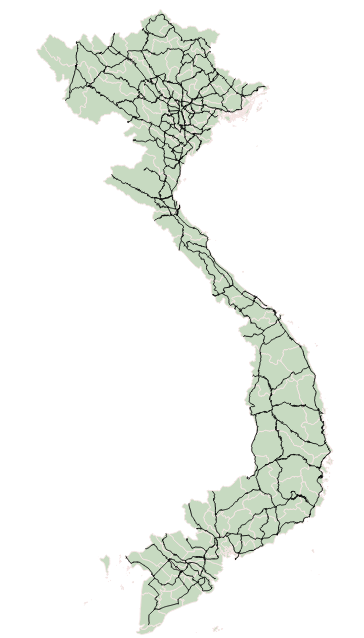
\includegraphics[width=0.5\textwidth]{figures/vietnamroad03.png} % second figure itself
		\caption[Dữ liệu đường bộ Việt Nam được đặt trên bản đồ địa chính]{dữ liệu đường bộ Việt Nam được đặt trên bản đồ địa chính, hiển thị bằng phần mềm QGIS.}
		\label{fig:vnhighway02}
	\end{minipage}
\end{figure}

Một số thông tin về dữ liệu GIS đường bộ Việt Nam:
\begin{itemize}
	\item Dữ liệu mô tả các đoạn đường quốc lộ trên lãnh thổ Việt Nam, tổng số có 2736 đoạn đường nhỏ.
	\item Mỗi doạn đường đều có các trường thuộc tính mô tả thông tin của đoạn đường đó, như tên đường, mã đường, độ đài đoạn đường, tốc độ tối đa.
\end{itemize}

\subsubsection{Phương pháp mô hình đồ thị cho dữ liệu GIS đường bộ Việt Nam}
Vì mạng giao thông là đối tượng thực tế, nên dữ liệu giao thông cũng giống với những dữ liệu thực tế khác, rất đa dạng và đa chiều. 
Tùy thuộc vào từng bài toán, với mục tiêu khác nhau, ta sẽ có một mô hình toán học phù hợp cho quá trình giải quyết bài toán đó.
Trong báo cáo này, tôi sử dụng mô hình toán học đơn giản là đồ thị vô hướng để mô hình mạng giao thông đường bộ Việt Nam. 

Nguyên tắc xây dựng mô hình đồ thị của mạng giao thông:
\begin{itemize}
	\item Mỗi đỉnh trong đồ thị, ứng với một nút giao thông,
	\item Mỗi cạnh nối hai đỉnh trong đồ thị tương ứng với một đoạn đường trên bản đồ. Các đường quốc lộ Việt Nam đều là đường hai chiều nên ta sử dụng đồ thị vô hướng để biểu diễn mạng giao thông.
	\item Các đỉnh và cạnh của đồ thị ngoài có định đanh duy nhất và chứa thông tin thu được từ dữ liệu GIS đường bộ Việt Nam.
	\item Mỗi đỉnh của đồ thị có hai trường thuộc tính kinh độ và vĩ độ của nút giao thông ứng với đỉnh đó.
	\item Mỗi cạnh của đồ thị chứa các thuộc tính của đoạn đường mà nó biểu diễn, ví dụ như tên đường, loại đường, độ dài hay tốc độ tối đa cho phép.
\end{itemize}

Chi tiết các bước xây dựng đồ thị đường bộ Việt Nam từ dữ liệu GIS được mô tả trong bảng \ref{table:graphcreation}:
%
\begin{table}[!h]
	\caption[Thủ tục xây dựng đồ thị đường bộ Việt Nam.]{Thủ tục xây dựng đồ thị đường bộ Việt Nam.}
	\begin{tabular}{ |m{15cm}| } 
		\hline
		\begin{enumerate}
			\item Đọc dữ liệu GIS đường bộ Việt Nam, trích lấy danh sách đối tượng đặc trưng (feature), gọi tắt là \textbf{FEAT\_LIST}. Mỗi đặc trưng đại diện cho một đoạn đường thực tế, được biểu diễn như một đường (polyline) - danh sách các điểm nằm trên đoạn đường đó. Mỗi đặc trưng cũng chứa các thuộc tính của đoạn đường đó.
			\item Tạo một đồ thị rỗng $G = (V,E), n(V) = 0$.
			\item Với mỗi đặc trưng trong \textbf{FEAT\_LIST}:
			\begin{itemize}
				\item Lấy thông tin tọa độ điểm đầu $P_0$ và điểm cuối $P_1$ của đặc trưng (đoạn đường) đó.
				\item Tương ứng với hai điểm $P_0$ và $P_1$, thêm hai đỉnh mới $u_0$ và $u_1$ vào đồ thị $G$. Tọa độ của các đỉnh chính là tọa độ của điểm tương ứng của đặc trưng.
				\item Tạo cạnh giữa $u_0$ và $u_1$ ứng với đoạn đường mà đặc trưng mô tả.
				\item Thêm các thuộc tính của đặc trưng vào cạnh $(u_0,u_1)$ vừa tạo.
				\item Lưu đồ thị $G$ dưới định dạng có thể đọc được bởi máy tính.
			\end{itemize}
		\end{enumerate}
		\\
		\hline
	\end{tabular}
	\label{table:graphcreation}
\end{table}

Bảng \ref{table:graphcreation} chỉ mô tả các bước cơ bản trong xây dựng đồ thị giao thông Việt Nam. Có rất nhiều trường hợp cần phải xử lý để thu được đồ thị đúng với mạng giao thông được dữ liệu GIS mô tả. Qua quá trình xử lý dữ liệu GIS xây dựng đồ thị giao thông, tôi rút ra một số chú ý:
\begin{itemize}
	\item Chỉ thêm những đỉnh có tọa độ mới vào đồ thị $G$. Nếu một hoặc hai đầu mút của một đoạn đường có tọa độ trùng với một đỉnh của đồ thị $G$, tức là tồn tại một đoạn đường được xử lý trước đó, có chung đầu mút với đoạn đường hiện tại. Khi đó, ta chỉ lấy ra định danh của các đỉnh đó chứ không tạo đỉnh mới. Sau đó tiếp tục thêm cạnh giữa các đỉnh ứng với đoạn đường đó.
	
	\item Xử lý giao nhau là một công đoạn quan trọng trong xây dựng đồ thị. Với những trường hợp một trong hai đầu mút của một đoạn đường $A$ lại nằm giữa một đoạn đường $B$ khác (trường hợp ngã ba), thì đoạn đường $B$ phải bị chia làm hai đoạn đường con $B_1$ và $B_2$ nối tiếp nhau. Hai đoạn đường con này có các thuộc tính giống với thuộc tính của đoạn đường $B$, trừ thuộc tính độ dài đoạn đường phải được tính lại cho mỗi đoạn đường.
	
	\item Khi xử lý tọa độ địa lý của các điểm, cần thống nhất về độ chính xác của tọa độ, tránh trường hợp quá trình làm tròn xảy ra gây sai lệch dữ liệu, như hai điểm rất gần nhau bị chập làm một; hay ngược lại hai điểm thực ra là một nhưng vì độ chính xác (ví dụ số chữ số phần thập phân) khác nhau nên lại bị coi là hai điểm khác nhau, có thể dẫn đến mất tính liên thông của đồ thị thu được.
	
	\item Một số dữ liệu địa lý được thu thập sử dụng hệ tọa độ địa lý cầu (Spherical Coordinates), trong đó đơn vị của tọa độ các điểm là độ. Hệ tọa độ này không cho phép tính khoảng cách giữa các điểm theo đơn vị mét. Vì vậy cần áp dụng một phép chiếu lên dữ liệu này, tùy vào vị trí địa lý của vùng dữ liệu cũng như phép chiếu được chọn. Kết quả của phép chiếu là tọa độ mới của tất cả các điểm, trong hệ tọa độ địa lý mới. Lúc đó việc tính toán khoảng cách thực tế mới được áp dụng.
\end{itemize}

Kết quả xử lý dữ liệu GIS để thu được đồ thị được biểu diễn trong hình \ref{fig:vnhighwaynet}. Các đỉnh của đồ thị được đặt vào các vị trí tương đối với nhau như trên địa lý.

\begin{figure}[!h]
	\centering
	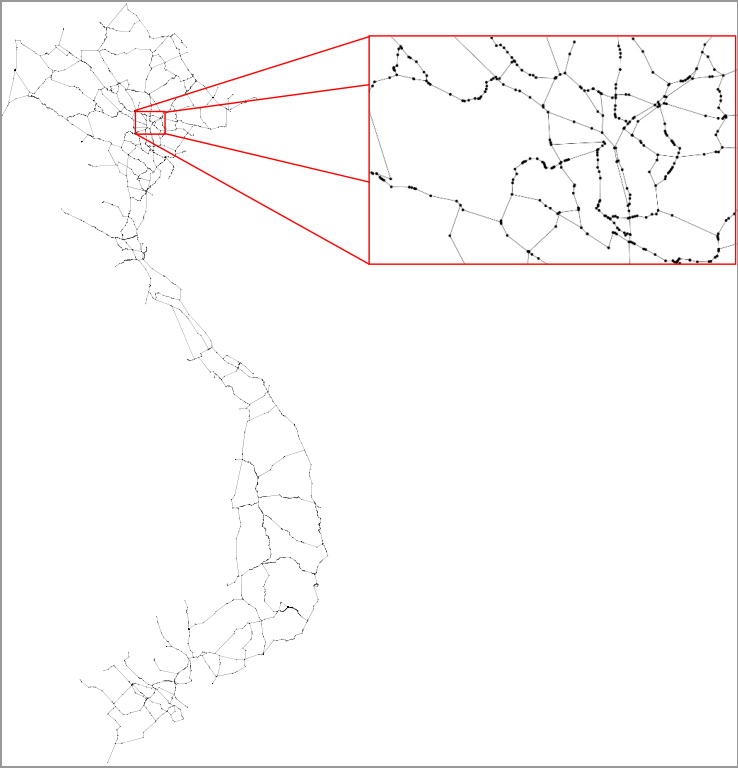
\includegraphics[scale=0.6]{figures/vnroadgraphtotaledit.png} 
	\caption[Đồ thị đường bộ Việt Nam]{Đồ thị đường bộ Việt Nam, tổng quan và chi tiết một vùng}
	\label{fig:vnhighwaynet}
\end{figure}
\subsection{Phân tích mạng đường bộ Việt Nam}
Hình \ref{fig:degreedist} biểu diễn biểu phân phối bậc của các đỉnh trong đồ thị mạng đường bộ Việt Nam. Trong dữ liệu GIS đường bộ Việt Nam có rất nhiều đoạn đường ngắn, nối tiếp nhau, của cùng một tên đường, nên ta có thể thấy là số đỉnh bậc 2 chiếm đa số trong phân phối bậc của đỉnh. Còn lại số đỉnh bậc 1, 3 và 4 của đồ thị khá hợp lý, khi có phân phối bậc tương tự với kết quả thu được trong phân tích mạng giao thông của Thụy Sĩ \cite{swissroad}. Số đỉnh bậc 3 và 4 chiếm đa phần nếu không tính các đỉnh bậc 2 sinh ra do dữ liệu chưa chuẩn, không có đỉnh bậc 5 và 6 nào trong đồ thị.

\begin{figure}[!h]
	\centering
	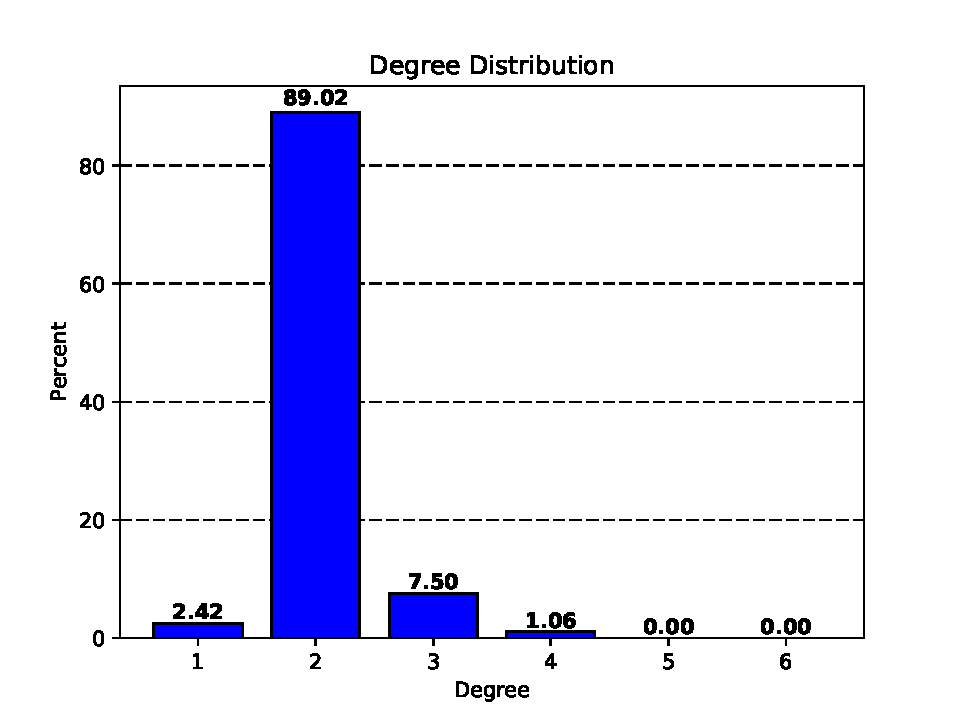
\includegraphics[scale=0.9]{figures/degreedist.pdf} 
	\caption[Phân phối bậc của đỉnh trong mạng đường bộ Việt Nam]{Phân phối bậc của đỉnh trong mạng đường bộ Việt Nam.}
	\label{fig:degreedist}
\end{figure}

Nếu không tính các đỉnh bậc 2, phân phối bậc của độ thị đường bộ Việt Nam sẽ có dạng như hình \ref{fig:degreedist2}.

\begin{figure}[!h]
	\centering
	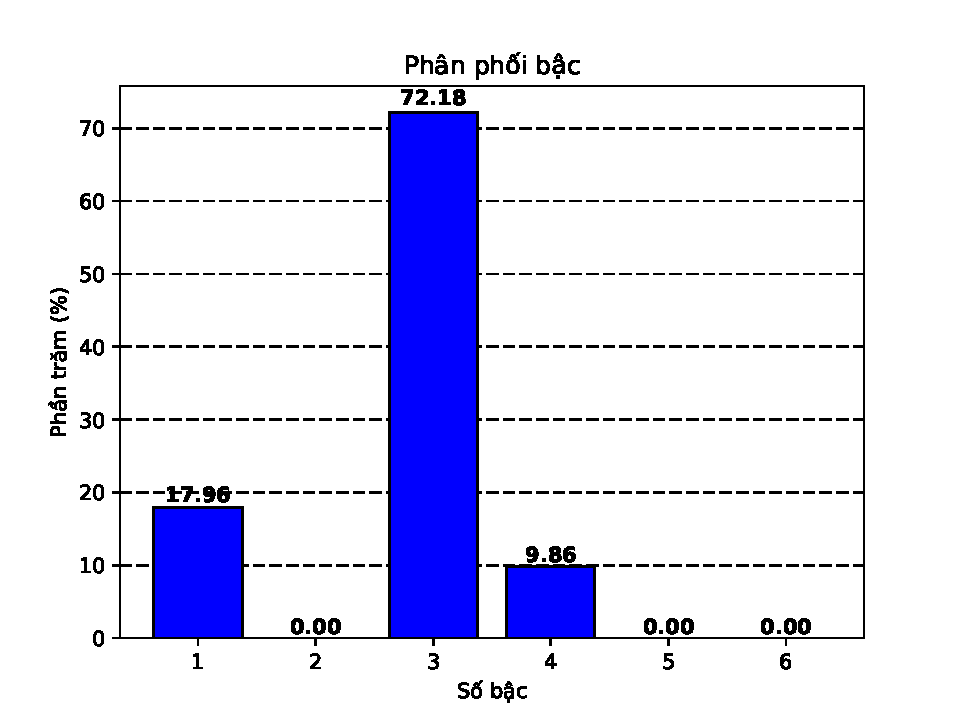
\includegraphics[scale=0.9]{figures/degreedist3.pdf} 
	\caption[Phân phối bậc của đỉnh trong mạng đường bộ Việt Nam khi loại bỏ đi các đỉnh bậc 2]{Phân phối bậc của đỉnh trong mạng đường bộ Việt Nam khi loại bỏ đi các đỉnh bậc 2.}
	\label{fig:degreedist2}
\end{figure}

Bảng \ref{table:measures} tổng hợp các chỉ số cơ bản của đồ thị:
\begin{table}[!h]
	\caption[Các chỉ số phân tích đồ thị đường bộ Việt Nam]{Các chỉ số phân tích đồ thị đường bộ Việt Nam}
	\centering
	\begin{tabular}{ |c|c| } 
		\hline
		Tên chỉ số & Giá trị \\ 
		\hline
		Bán kính & 193\\
		Đường kính & 386\\ 
		Độ dài đường đi trung bình không có trọng số & 132.09448\\
		Độ dài đường đi trung bình dựa trên độ dài đoạn đường & 885.35909 km\\ 
		Hệ số phân cụm trung bình & 0.003\\
		Mật độ của đồ thị & 0.001\\ 
		\hline
	\end{tabular}
	\label{table:measures}
\end{table}

Các chỉ số phân tích trong bảng \ref{table:measures} đều cho thấy đồ thị đường bộ Việt Nam có tính chất của đồ thị thưa, với bán kính và đường kính lớn, tức là cần đi qua nhiều đỉnh, đi đoạn đường dài, để đến được các đỉnh khác trong đồ thị. Hệ số phân cụm trung bình thấp và mật độ của đồ thị thấp cũng thể hiện điều này.
Để có thêm thông tin về tính chất của mạng giao thông đường bộ Việt Nam, ta xét đến một chỉ số quan trọng, chính là chỉ số trung tâm trung gian.

\subsubsection{Phân tích chỉ số trung tâm trung gian}
Trong mạng giao thông, ý nghĩa trực tiếp của chỉ số trung tâm trung gian, vốn được tính dựa trên số lượng đường đi ngắn nhất đi qua đỉnh hay cạnh đó, chính là mức độ tải mà mỗi đỉnh hay cạnh phải chịu (node load, link load), với giả thiết rằng các phương tiện tham gia giao thông đều chọn đường ngắn nhất để đi.

Trong báo cáo này, các đường đi ngắn nhất và chỉ số trung tâm trung gian được tính dựa trên trọng số hay chi phí là độ dài của các đoạn đường, để phản ánh thực tế cách đi chuyển của các phương tiện, hơn là coi mỗi cạnh trong đồ thị đều có trong số là 1.

Hình \ref{fig:betweeness} biểu diễn kết quả tính toán chỉ số trung tâm trung gian cho các đỉnh của đồ thị đường bộ Việt Nam, được thể hiện dựa trên quan hệ tương đối giữa kích thước của các đỉnh trong đồ thị, các đỉnh có chỉ số trung tâm trung gian cao sẽ có bán kính lớn, và ngược lại.
Ta có thể thấy là những nút giao thông có chỉ số trung tâm trung gian cao, hay mức độ tải phải chịu lớn, thường nằm trên các trục đường quốc lộ chính, nối các tỉnh với nhau. Ví dụ như các nút giao thông trên đường Quốc Lộ 1 dọc từ thành phố Hà Nội đến Đà Nẵng đều có chỉ số trung tâm trung gian cao, trong khi trục đường quốc lộ song song với Quốc Lộ 1 lại không có chỉ số trung tâm trung gian cao như vậy.

Tương tự, ta có thể thấy tại khu vực Tây Nguyên, đường Quốc Lộ 14 lại là tuyến đường có các nút giao thông với chỉ số trung tâm trung gian cao. Ở khu vực Nam Bộ, đường Quốc Lộ 1 lại có chỉ số trung tâm trung gian cao trở lại, thể hiện sự kết nối giữa các tỉnh khu vực Tây Nguyên và các tỉnh khu vực Nam Bộ.

\begin{figure}
	\centering
	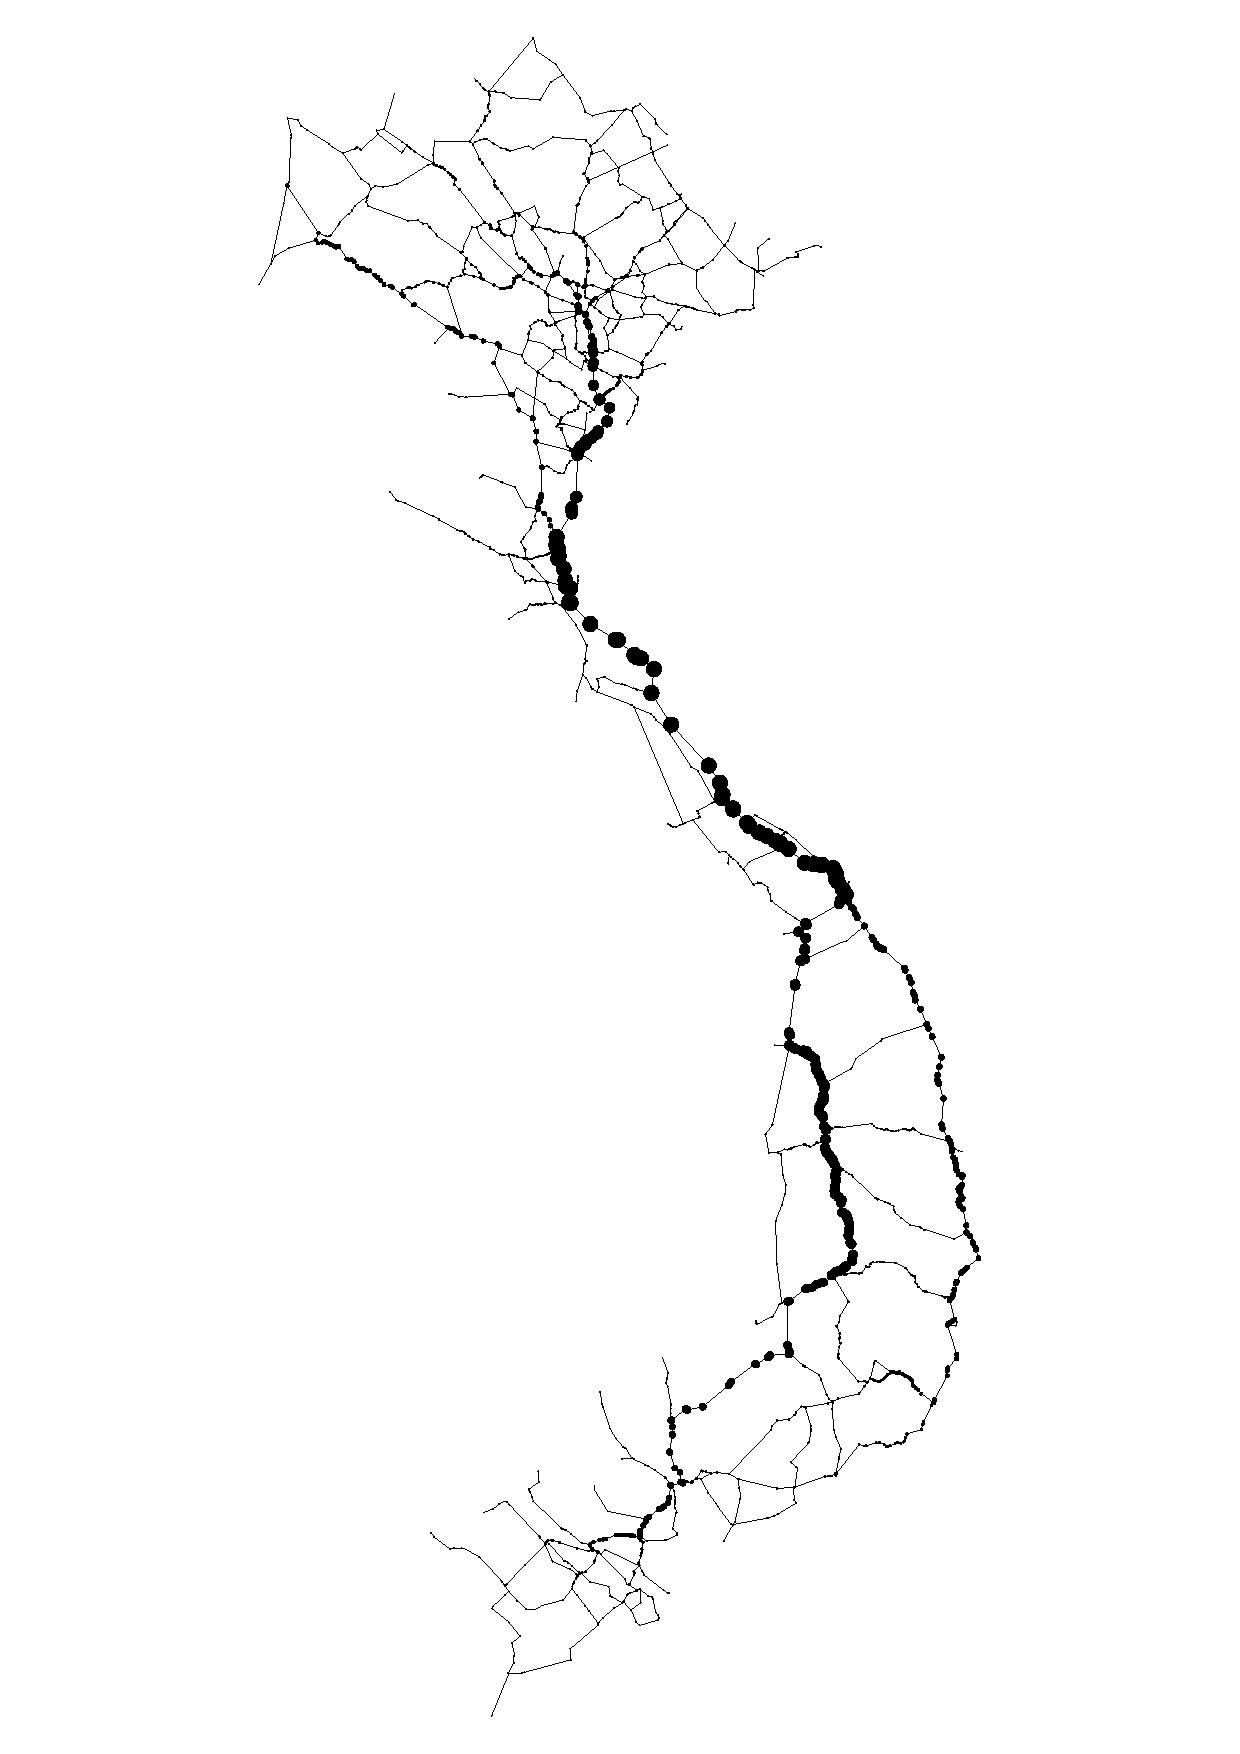
\includegraphics[scale=0.7]{figures/vietnamroadbetweeness.pdf} 
	\caption[Đồ thị đường bộ Việt Nam biểu diễn chỉ số trung tâm trung gian]{Đồ thị đường bộ Việt Nam biểu diễn chỉ số trung tâm trung gian}
	\label{fig:betweeness}
\end{figure}

\begin{figure}
	\centering
	\begin{subfigure}{.5\textwidth}
		\centering
		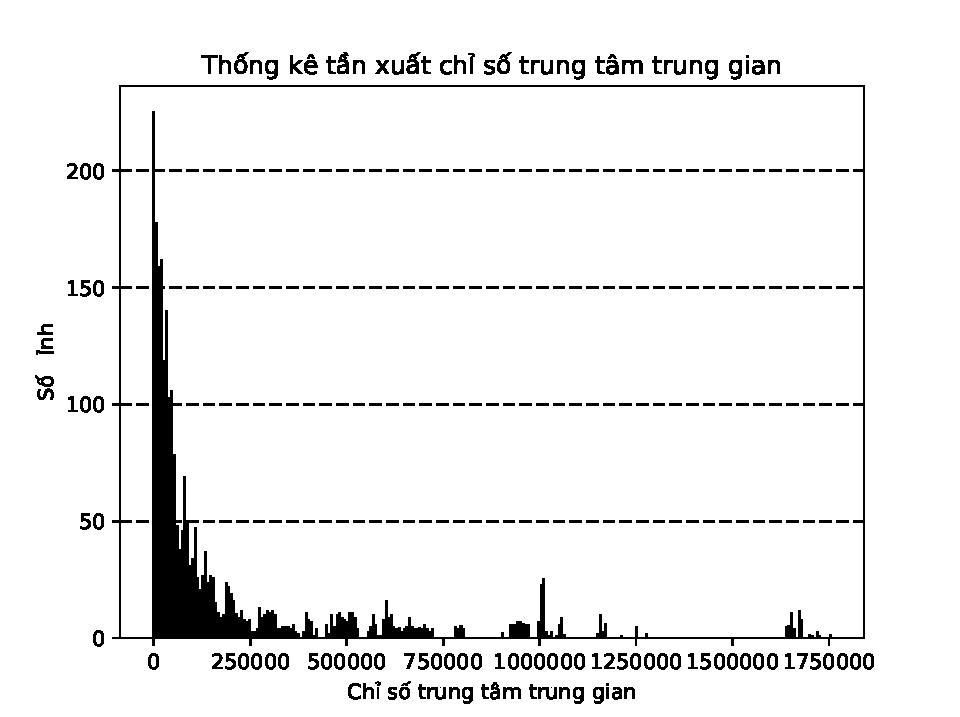
\includegraphics[scale=0.5]{figures/betweeness_dist.pdf}
		\caption{Chỉ số trung tâm trung gian cạnh}
		\label{fig:betweenessdist}
	\end{subfigure}%
	\begin{subfigure}{.5\textwidth}
		\centering
		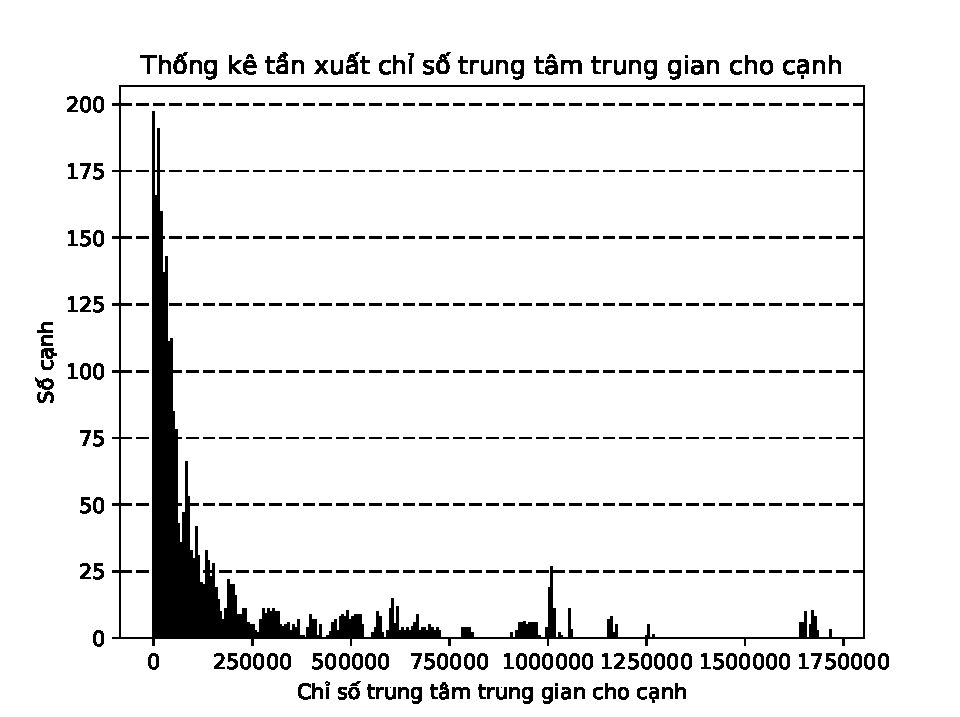
\includegraphics[scale=0.5]{figures/betweeness_edge_dist.pdf}
		\caption{Chỉ số trung tâm trung gian cạnh}
		\label{fig:betweenessedgedist}
	\end{subfigure}
	\caption{Biểu đồ tần xuất chỉ số trung tâm trung gian đồ thị đường bộ Việt Nam}
	\label{fig:between}
\end{figure}

Về mặt phân phối, ta có thể thấy trong hình \ref{fig:between}, hai biểu đồ biểu diễn tần xuất (histogram) của chỉ số trung tâm trung gian của các đỉnh \ref{fig:betweenessdist} và các cạnh \ref{fig:betweenessedgedist} của đồ thị đường bộ Việt Nam. Có thể nhận thấy rằng trong cả hai biểu đồ, số lượng đỉnh (cạnh) có chỉ trung tâm trung gian thấp chiếm đa số, còn số lượng đỉnh có chỉ số trung tâm trung gian cao và rất cao là rất thấp.

%%%%%%%%%%%%%%%%%%%%%%%%%%%%%%%%%%%%%%%%%%%%%%%%%%%%%%%%%%%%%%%%%%%%%%%%%%%%%%%%

%\newpage
%\section{Ứng dụng lý thuyết đồ thị trong phân tích mạng giao thông Việt Nam}
%\subsection{Các khái niệm trong giao thông vận tải}
%\subsection{Khoa học thông tin địa lý (GIS)}
%\subsection{Mô hình hóa dữ liệu GIS đường bộ Việt Nam bằng đồ thị}
%\subsubsection{Dữ liệu GIS về giao thông đường bộ Việt Nam}
%\subsection{Những đặc trưng cơ bản trong phân tích đồ thị}
%\subsection{Phân tích mạng đường bộ Việt Nam}
%\subsubsection{Phân tích các chỉ số cơ bản}
\newpage
\fancyhead[R]{Kết luận}
\section{Kết luận}
Trong báo cáo này, tôi đã trình bày hai vấn đề: ứng dụng lý thuyết đồ thị vào dịch tễ học và ứng dụng trong phân tích mang giao thông đường bộ Việt Nam. 

Bài toán tìm tập độc lập cực đại được ứng dụng trong tiêm phòng ngăn ngừa bệnh dịch lây lan trong mạng truyền nhiễm. Nhưng trong thực tế, còn rất nhiều vấn đề nảy sinh nếu áp dụng những thuật toán này vào thực nghiệm. Có thể kể đến như: (1) việc xây dựng được mạng dịch tễ là rất khó và phức tạp, (2) cấu trúc mạng dịch tễ có thể thay đổi theo từng ngày, khi mỗi ngày có rất nhiều ca mắc bệnh mới cũng như khỏi bệnh, (3) quá trình tiêm phòng cho một cộng đồng không thể làm xong trong một thời gian ngắn, trong thời gian tiêm phòng cấu trúc mạng thay đổi có thể làm kế hoạch tiêm phòng hoàn toàn thất bại. Cần nhiều nghiên cứu hơn nữa để thực tế hóa phương pháp tiêm phòng sử dụng tập độc lập này.

Bài toán phân tích mạng giao thông Việt Nam của tôi mới chỉ bó hẹp trong một loại chỉ số trung tâm, còn rất nhiều những phương pháp phân tích mạng giao thông khác và những bài toán khác như tìm ra những tuyến đường hay xảy ra tắc nghẽn giao thông, áp dụng mô hình cung cầu trong mạng giao thông để phân tích những vùng kinh tế dựa trên lưu lượng giao thông giữa các vùng, tính toán khả năng chịu tải của hệ thống giao thông khi có sự cố xảy ra trên một số tuyến đường.

Nói chung, ứng dụng lý thuyết đồ thị vào các vấn đề thực tế còn rất nhiều bài toán hay và khó. Trong những nghiên cứu tiếp theo, tôi mong sẽ có thể tiếp tục phát triển những ứng dụng này.

Do năng lực và thời gian có hạn, báo cáo còn nhiều sai sót, mong nhận được góp ý thêm, tôi xin chân thành cảm ơn.
\newpage
%%%%%
\printindex
%%%%%
\newpage
\begin{thebibliography}{9}
	\bibitem{graphtextbook}
	Douglas B. West,
	\textit{Introduction to graph theory, Second Edition},
	Prentice Hall, ISBN: 9780130144003, 2001
	%
	\bibitem{yannakakis01}
	Yannakakis M.,
	"Node-Deletion Problems on Bipartite Graphs",
	SIAM Journal on Computing 10 (2 1981), pp. 310–327. ISSN: 0097-5397.
	%
	\bibitem{graphclasses}
	ISGCI: Information System on Graph Class Inclusions v2.0. "List of Small Graphs." \href{http://www.graphclasses.org/smallgraphs.html}{http://www.graphclasses.org/smallgraphs.html}.
	%
	\bibitem{swissroad}
	Alexander Erath, Michael Löchl, Kay W. Axhausen,
	"Graph-Theoretical Analysis of the Swiss Road and Railway Networks Over Time", 
	Networks and Spatial Economics,
	September 2009, Volume 9, Issue 3, pp 379–400
	%
	\bibitem{MIS}
	Ngoc C. Lê. Christoph Brause and Ingo Schiermeyer,
	"ON SEQUENTIAL HEURISTIC METHODS FOR THE MAXIMUM INDEPENDENT SET PROBLEM",
	Discussiones Mathematicae, Graph Theory 37 (2017) pp. 415–426
	%
	\bibitem{MINAlgorithm}
	Murphy, O. J.
	"Lower Bounds on the Stability Number of Graphs Computed in Terms of Degrees", Discrete Mathematics 90 (2 1991), pp. 207–211. issn: 0012-365X. 
	\bibitem{MAXAlgorithm}
	Griggs, J. R.
	"Lower Bounds on the Independence Number in Terms of the Degrees",
	\textit{Combinatorica} 1 (2 1981), pp. 169–197.
	%
	\bibitem{VOAlgorithm}
	Mahadev, N. V. R. and Reed, B. A.
	"A Note on Vertex Order for Stability Number",
	\textit{Journal of Graph Theorey} 30 (2 1999), pp. 113–120.
	%
	\bibitem{alpharedundan}
	Brandstädt, A. and Hammer, P. L.
	\textit{"A Note on $\alpha$-redundant Vertices in Graphs"},
	Discrete Applied Mathematics 108 (3 2001), pp. 301–308.
	%
	\bibitem{alpharedudant2}
	Gerber, M. U. and Lozin, V. V.,
	"Robust Algorithms for the Stable Set Problem",
	Graphs and Combinatorics 19 (3 2003), pp. 347–356. ISSN: 1435-5914.
	%
	\bibitem{BasicEpid}
	R. Bonita, R. Beaglehole, Tord Kjellström,
	\textit{Basic epidemiology},
	World Health Organization 2009, second edition.
	%
	\bibitem{centrali01}
	Freeman, L.C.
	"Centrality in social networks: conceptual clarification",
	Social Networks, (1979) pp. 215-239.
	%
	\bibitem{centrali02}
	Freeman, L. C.
	"A set of measures of centrality based on betweenness",
	Sociometry, (1977) Vol. 40, No. 1, pp. 35-41.
	%
	\bibitem{centrali03}
	Sabidussi, G. 
	"The centrality index of a graph",
	 Psychometrika, Vol. 31 , pp. 581-603.
	 %
	 \bibitem{efficiency01}
	 Latora, V. and M. Marchiori,
	 "Efficient beahviour of small-world networks",
	 "Physical Review Letters" (2001), Vol. 87.
	 %
	 \bibitem{efficiency02}
	 Latora, V. and M. Marchiori, 
	 "Is the Boston subway a small-world network?",
	 Physica A (2002), Vol. 314 , pp. 109–113.
	 %
	 \bibitem{complexnetwork}
	 Kayhan Erciyes,
	 \textit{Complex Networks: An Algorithmic Perspective},
	 CRC Press, isbn: 1466571667, 9781466571662, 2014.
	 %
	 \bibitem{randnet}
	 P. Erdos andA. Renyi.
	 "On random graphs",
	 Publicationes Mathematicae, pp. 290-297, 1959.
	 %
	 \bibitem{geospatialbook}
	  Erik Westra,
	 \textit{Python Geospatial Development - Second Edition},
	 Packt Publishing, ISBN: 978-1-78216-152-3.
	 %
	 \bibitem{qgis}
	 \href{http://www.qgis.org/en/site/}{http://www.qgis.org/en/site/}
	 %
	 \bibitem{neworkx}
	 \href{https://networkx.github.io/}{https://networkx.github.io/}
	 %
	 \bibitem{gephi}
	 \href{https://gephi.org/}{https://gephi.org/}
	 
\end{thebibliography}

\end{document}